% NSF proposal generation template style file.
% based on latex stylefiles written by Stefan Llewellyn Smith and
% Sarah Gille, with contributions from other collaborators.
%
\documentclass{nsfproposal}

\usepackage[super,sort&compress]{natbib}
\usepackage{longtable}
\usepackage{booktabs}
\usepackage{todonotes}
\usepackage{hyperref}
\usepackage{bibentry}
\usepackage{textcomp}
\usepackage{wrapfig}
\usepackage{soul}
\setuldepth{1}
\usepackage[most]{tcolorbox}
\usepackage[skip=5pt]{caption}
\usepackage[absolute]{textpos}
\usepackage{gensymb}
\textblockorigin{2 in}{2 in}
\usepackage{caption}
\captionsetup[figure]{font=small,labelfont=small}

\setlength{\TPHorizModule}{\textwidth}
\setlength{\TPVertModule}{\textheight}
\newcommand\highlight[1]{\ul{\textit{#1}}}

\title{Role of nanominerals on photochemical derived atmospheric NH\textsubscript{3} and N\textsubscript{2}O}
%%^^If we could get this to one line it would buy a little space on the first page.

%Fundamental understanding of the photocatalytic interaction between environmentally-relevant oxide interfaces and the nitrogen cycle
%Investigation of photocatalytic nitrogen fixation and redox chemistry at environmentally-relevant oxide interfaces
%Fundamental investigation of environmentally-relevant oxide photocatalysts on the nitrogen cycle

\makeatletter
\newcommand{\LeftHeader}{}
\newcommand{\MiddleHeader}{}
\newcommand{\RightHeader}{Georgia Institute of Technology}
\newcommand{\LeftFooter}{Project Summary}
\newcommand{\PageLimit}{1}
\newcommand{\toPageLimit}{ of \PageLimit}
% Commands for defining headers. The tex file for each document should re-define Document and PageLimit.

\DeclareTextFontCommand{\emph}{\bfseries\em}
%Make emph bold+italic

%Convenience "to do" commands
\newcommand{\todomarta}[1]{\todo[color=green]{Hatzell: #1}}
\newcommand{\todoaj}[1]{\todo[color=blue]{Medford: #1}}

\newcommand{\TIO}{TiO$_2$}
\newcommand{\NN}{N$_2$}
\newcommand{\NH}{NH\textsubscript{3}}
\newcommand{\NO}{N\textsubscript{2}O}
\newcommand{\mathplus}{+} %annoying bibtex thing
%convenience functions

\def\baselinestretch{1}

\begin{document}

%\renewcommand{\LeftFooter}{Cover Sheet}
\renewcommand{\PageLimit}{0} %0 page limit puts no "of X" in page numbers

\begin{center}
\textbf{\textsf{\large Routing Sheet Info}} \\*[1.5mm]
\end{center}

\begin{itemize}
\item \textbf{Title:}  \@title
\item \textbf{Total Budget:} 
\$330,000
\item \textbf{Georgia Tech Budget:} 
\$330,000
\item \textbf{Period of Performance:} 
April 2017 - April 2020
\item \textbf{Keywords:} 
nitrogen cycle, photocatalysis, fertilizers, titania
\item \textbf{PI:} 
Andrew J. Medford
 \begin{itemize}
 \item \textbf{Affliation:} Georgia Tech ChBE
 \item \textbf{NSF ID:}  000716383
 \end{itemize}
\item \textbf{Co-PI:} 
Marta C. Hatzell
 \begin{itemize}
 \item \textbf{Affliation:} Georgia Tech Mechanical Engineering
 \item \textbf{NSF ID:}  000704894
 \end{itemize}
\item \textbf{Co-PI:} 
Carsten Sievers
 \begin{itemize}
 \item \textbf{Affliation:} Georgia Tech ChBE
 \item \textbf{NSF ID:}  000512515
 \end{itemize}
 
\item \textbf{Special Review Criteria:} Bold if applicable
\begin{itemize}
\item \textbf{None}
\item Human Subject Research?
\item Vertebrate Animals? 
\item Recombinant DNA?
\item Biological agents:
\item Physical Agents. 
\item Materials Transfer Agreement (MTA)
\item Professional Education Program 
\item Subaward(s) are proposed
\item Teaming Agreement
\item Export of info or materials to another country
\item Foreign sponsor or collaborator, or will be performed in whole \item or in part outside the U.S.
\item Contract anticipated to contain restrictions on publication or \item the use of Foreign Nationals
\item Involves the use of pre-existing (background) intellectual \item property Georgia Tech’s Third Party’s –explain in comments section.
\item A member of the research team has a Significant Financial Interest (SFI) related to this project. 
\end{itemize}
\end{itemize}

%\setcounter{page}{1}

%\listoftodos
%\newpage
%\setcounter{page}{1}

% Use includes for each document to make writing easier. Starting names with a number allows keeping them organized in the project folder
\renewcommand{\LeftFooter}{Project Summary}
\renewcommand{\PageLimit}{1} %0 page limit puts no "of X" in page numbers
\vspace{-15pt}

\textbf{Summary:} In natural environments, a range of nanominerals, dissolved metals and organic compounds contribute to the natural abiotic chemical nitrogen cycle. Nanomaterial based semiconductors are widely abundant in global sands and soils. The role these natural nanominerals play in the nitrogen cycle is unknown. Throughout the last century significant evidence has been presented suggesting that  abiotic nitrogen-based transformations are significant. Specifically, abiotic solar driven processes such as nitrogen reduction and oxidation, ammonia oxidation and nitrate reduction have all been demonstrated on environmentally abundant minerals and metals. These processes are central to the nitrogen cycle, and are analogous to the well-studied biological processes: nitrogen fixation, nitrification and denitrification. Furthermore, these abiotic transformations have all been demonstrated  under environmentally relevant conditions (ambient pressure and temperature).  Here, through the use of first-principles calculations, photocatalytic testing, and in situ spectroscopic tools, the chemical mechanisms and physical phenomena that enable gas-phase photocatalytic nitrogen fixation and ammonia oxidation environmental settings. This fundamental understanding will provide insight into the role of terrestrial sands and minerals on the natural nitrogen cycle, providing a foundation for more accurate models of nutrient fluxes in terrestrial settings. Furthermore, the findings will elucidate the interactions between oxide surfaces, photons, and nitrogen compounds that enable these transformations. This knowledge will lay the groundwork for future technologies to manage and control the nitrogen cycle in a more sustainable way.

Intensification of agriculture and rising emissions from the burning of fossil fuels has led to a 3-5x increase in reactive nitrogen emissions (N$_2$O,NH$_3$,NO$_x$) over the past century. 

\textbf{Intellectual Merit:} The work will seek to unambiguously determine the role of natural nano-minerals play in enabling key photocatalytic nitrogen-based transformation (nitrogen fixation, nitrification, and ammonification). 

%Specifically, we will investigate three core hypotheses: i) the ratio of titania to hematite controls the ratio of ammonium/nitrate during fixation and nitrification, ii) optimum nitrogen photofixation occurs at moderate temperatures and humidities (35 C and 50\%) and iii) surface impurities are critical for enabling photocatalytic nitrogen fixation. The knowledge gained from testing these hypotheses will significantly impact the understanding of the global abiotic nitrogen cycle, which has the potential to alter our understanding of soil nutrition in a range of environments. This will be the first work to explore this enigmatic phenomenon with modern techniques, and will provide key insight into the broader importance of the emerging field of photogeochemistry in the natural nutrient cycle. 


%Furthermore,this work will advance knowledge in the fields of surface science and catalysis by establishing a molecular-level understanding of photocatalytic nitrogen based transformation on titania. This will be the first time this system has been studied with applied bias, and the first photocatalytic nitrogen fixation study using in situ spectroscopy (FTIR, XPS). These unique experiments will be coupled with density functional theory (DFT) calculations to enable new atomic-scale insights into the surface intermediates.  Gaining a molecular-level understanding of the photocatalytic nitrogen fixation process on titania will be a foundation step to the rational optimization and design of photocatalysts that can enable more sustainable fertilizer production processes.

\textbf{Broader Impacts:} Managing the nitrogen cycle has been deemed a critical component of the food-energy-water (FEW) nexus, as control over the composition of reduced and oxidized nitrogen species in soils is needed for food production. Furthermore, with growing populations in a range of centralized and decentralized regions, understanding nutrient transformations processes will only grow in importance. The critical first step in managing the nitrogen cycle is to define the magnitude and mechanisms of each N-based transformation. This is historically difficult, as the  nitrogen cycle is known to be the most complex biogeochemical nutrient cycle.  The proposed broader impact of this work will specifically aim to determine how solar-driven abiotic N-transformations contribute to nutrient cycles. 

The impact of the work will be enhanced by outreach and educational efforts. The findings will be highlighted through a publicly accessible website and YouTube videos that demonstrate key findings and suggest simple experiments that can be performed with household items. Furthermore, the work will be the basis of a capstone project through Georgia Tech's Food-Energy-Water initiatives enabled through the Serve-Learn-Sustain program. This capstone project will explore scale-up challenges and engage undergraduate seniors from a range of academic disciplines including engineering and social sciences. The project will seek to establish a holistic view of the role of photocatalytic nitrogen fixation on the current environment and future chemical processes.



% * <marta.hatzell@me.gatech.edu> 2016-10-08T19:22:22.067Z:
%
% we may not want to bring up nitrate and water pollution issues. I get why, but since we are not directly targeting this issue it might be more confusing to a reviewer. the INFEWS call clearly states that alternative fertilizer production is an area of interests, so we should not have to worry about the connection to much.I removed the statement "Over fertilization can also lead to nitrate pollution of the groundwater tables.  

% overall the connections to broader impacts in text are good here"
%
% ^.
%The impact of the work will be enhanced by outreach and educational efforts. The findings will be highlighted through a publicly accessible website and YouTube videos that demonstrate key findings and suggest simple experiments that can be performed with household items. Furthermore, the work will be the basis of a capstone project through Georgia Tech's Food-Energy-Water initiatives enabled through the Serve-Learn-Sustain program. This capstone project will explore scale-up challenges and engage undergraduate seniors from a range of academic disciplines including engineering and social sciences. The project will seek to establish a holistic view of the role of photocatalytic nitrogen fixation on the current environment and future chemical processes.

\newpage

\setcounter{page}{1}
\renewcommand{\LeftFooter}{Project Description}
\renewcommand{\PageLimit}{15}
\begin{center}
\textbf{\textsf{\large \@title}} \\*[2mm]
\end{center}

\section{Overview \& Motivation} 
\vspace{1mm}


The main research objective of this proposal is to understand how photocatalytic earth-abundant nanominerals in soils and sands contribute to reactive nitrogen (NH\textsubscript{3}  and N\textsubscript{2}O) emissions into the atmosphere. Atmospheric \NH\hspace{.5mm} and \NO\hspace{.5mm} are well known environmental pollutants which are increasing largely due to anthropogenic activities associated with the agriculture (Fig \ref{fig:N2cycle} - top). These gases are emitted at a slower rate than CO\textsubscript{2}; however, are significantly more harmful to the environment.  For instance, \NO\hspace{.5mm} has a global warming potential of 298 and \NH\hspace{.5mm} allows for the formation of fine \begin{wrapfigure}{r}{0.33\textwidth}
\centering
\vspace{-1mm}
\fbox{\includegraphics[width=0.33\textwidth]{scripts/figures/N2_redox_ladder_abioticReactions2}}
\caption{(a) Agricultural related NH\textsubscript{3} and N\textsubscript{2}O emissions\cite{doane2017abiotic}. (b) Nitrogen redox ladder with relevant reactions and mineral band gaps indicated\cite{Medford_2017}.}
\label{fig:N2cycle}
\vspace{-2mm}
\end{wrapfigure}aerosol nitrates (NH\textsubscript{4}NO\textsubscript{3}) 
which contribute to increased atmospheric particulate matter (PM) which is hazardous to human health\cite{makar_2009}. This increase in nitrogen based emissions results in an imbalance in the nitrogen cycle, and is one reason why the National Academy of Engineering has listed, ``Managing the nitrogen cycle'' as one of the Grand Challenges of the next century. 


%The nitrogen cycle is almost exclusively centered around microbial nitrogen-based transformation. While microorganisims play a large role in mediating the nitrogen cycle, numerous lab demonstrations show that nearly every biotic reaction is possible through photochemical abiotic-based transformation on mineral catalyst. Notably, photochemical nitrification\cite{DHAR_1932,DHAR_1933,DHAR_1934,mclean1965reactions,kebede2013photooxidation}, nitrogen fixation \cite{dhar1941new,DHAR_1944,Schrauzer1977}, and denitrification \cite{cunningham1971reactions,blyholder1971photocatalytic} are noted to occur in natural settings under ambient conditions (see Fig. \ref{fig:N2cycle})a \cite{doane2017abiotic}. This raises the key question regarding if these lab-demonstrated reactions can occur in the environment.  The \textbf{central hypothesis of the proposed work is that earth abundant oxides in concert with sulfides do aid in mediating the abiotic nitrogen cycle}. 



%The nitrogen cycle is critical for life, as all living organisms need nitrogen to build amino acids, protein and tissue. It is also well recognized that human civilization is reliant on our ability to manage the nitrogen cycle in a way that allows for the production of enough nutrients to feed our growing population\cite{Galloway_2004}. This was even acknowledged by the National Academy of Engineering, which recently stated that managing the nitrogen cycle will be one of the Grand Challenges of the next century. However, in order to begin to manage the nitrogen cycle, we must fully understand all relevant transformations. Measuring and tracking these transformations has been a challenge, as the biogeochemical nutrient cycle includes nine possible intermediates, with oxidation states ranging from -3 to +5. For this reason, the nitrogen cycle is often deemed the ``most advanced biogeochemical cycle''\cite{stein2016nitrogen}. While significant progress has been made in describing the nitrogen cycle, nearly all terrestrial nitrogen transformations are still solely attributed to five biotic processes (nitrification, denitrification, fixation, ammonification, and anammox)\cite{Howard_1996}. 

Most agricultural related nitrogen emissions are largely thought to be due solely to microbial activities such as nitrogen fixation (\NH) and denitrification (\NO), and fertilizer volatilization. However, numerous abiotic solar-driven nitrogen transformation have been shown to be catalytic possible using earth-abundant photocatalytic nanominerals\cite{doane2017abiotic}. Photocatalytic nanominerals are widely abundant in soils and sand and exist primarily as oxides. The various minerals differ in the compositions and type of metals (Fe,Ti,Zn,W,Sr) contained within the crystal lattice which contribute to minerals with different band gaps and band edge (conduction and valance) locations (Fig \ref{fig:N2cycle}-bottom). Only a handful of research studies have been conducted to evaluate the activity of photocatalytic nanominerals, the preliminary evidence suggests that they are active for various nitrogen based transformation. For instance,  photonitrification\cite{DHAR_1932,DHAR_1933,DHAR_1934,mclean1965reactions,kebede2013photooxidation}, photofixation (nitrogen fixation) \cite{dhar1941new,DHAR_1944,Schrauzer1977}, and photodenitrification \cite{cunningham1971reactions,blyholder1971photocatalytic} have been confirmed to take place in natural settings under ambient conditions\cite{doane2017abiotic}. \textbf{There however have been no studies to investigate equilibrium partitioning of these photochemically derived intermediates and products between soils and air}. This has global importance, as documenting all emissions sources is necessary in order to develop robust climate models, and engineer solutions to mitigate the imbalance in the nitrogen cycle. Therefore, we aim to explore how these reactions contribute to atmsopheric emissions through the following research questions and hypotheses:  


\vspace{2mm}

\begin{enumerate}[label=\textbf{RQ\arabic*.}]
        
        %\item \textbf{How do photocatalytic oxides contribute to atmospheric NH\textsubscript{3} and NO\textsubscript{x}?}
      
        
       % \highlight{Hypothesis:} Sulfides photo-reduced N\textsubscript{2} to \NH\hspace{0.5mm} and oxides photo-oxidize  N\textsubscript{2} to produce \NO.
       
        \item \textbf{What effect do mineral properties (size, phase, facet, metal) play on photocatalyzed NH\textsubscript{3} and NO\textsubscript{x} emissions?}
      
        
                %\vspace{1mm}
                \item \textbf{What role does soil acidity play in promoting photocatalyzed reactions?}
                
                 \highlight{Hypothesis:} Photochemical reactions in alkaline soils promote the formation of \NO\hspace{0.5mm} and photochemical reactions in semi-dry acidic soils promote the formation of \NH.
        
    %    \highlight{Hypothesis:} Oxygen and sulfide based vacancies are active sites for dinitrogen but not nitrate.
          % \vspace{2mm}
          
        
            %  \vspace{1mm}
                \item \textbf{How does the solar irradiation properties (intensity, wavelength) impact emissions?}
        
       \highlight{Hypothesis:} Photochemimcal production of \NO\hspace{0.5mm} is produced at all wavelengths, while photochemical production of \NH\hspace{0.5mm} only is produced under UV illumination.
          % \vspace{1mm}
          
          
       % \item \textbf{How does atmospheric carbon (CO\textsubscript{2}) and soil carbon (organic) concentration impact photochemical N-transformations?}
        
       % \highlight{Hypothesis:} Increased atmospheric and soil carbon concentration results in an increased rate ammonia produced through enhancing photocatalytic-driven mineralization.  
        %   \vspace{2mm}
 
        
\end{enumerate}




\section{Technical Background}
\vspace{1mm}
\vspace{1mm}
\subsubsection*{Nitrogen Photochemistry and the Lithosphere} 
\vspace{1mm}

Photochemical nitrogen transformation were initially pioneered by a prominent Indian soil scientist, N.R. Dhar, in the 1930-40s \cite{DHAR_1932}. Dhar and colleagues' early work focused on illuminating sterile soils (no bacteria) with known ammonia salts. These early works, while far from conclusive, hinted that the rate of abiotic ammonia oxidation (nitrification) increased in the presence of sunlight.These results remained unverified until 1977, when Schrauzer and Guth also began to investigate this process on natural minerals\cite{Schrauzer1977,schrauzer1979nitrogen}. They restricted their focuses to Fe-doped titania and desert sands. Initially they collected common rocks, clays and sands. Results from controlled photocatalyic testing performed under sun-light indicated that \emph{common rocks did not exhibit high activity} for photofixation of nitrogen, but that \emph{sands were active}. Despite these initial findings, modern experimental and theoretical techniques have yet to be applied to the abiotic soil-nitrogen cycle, and no studies have looked at any additional photocatalytic processes beyond nitrogen fixation. However, these early works did try to quantify to potential impact of this point-source, and estimated that as much as \textcolor{red}{X\%} of all fixed nitrogen could come from photocatalyzed reactions. Despite this interesting finding, phtocatalyzed production of \NH\hspace{1mm} and \NO\hspace{1mm} are not included in any environmental emissions inventories. 





\vspace{1mm}
\subsubsection*{Nitrogen Photochemistry and the Atmospheric}
\vspace{1mm}

Nitrogen-based photochemical transformations in atmospheric sciences has been largely  restricted to understanding the fate of emitted pollutants (\NH, \NO, NO\textsubscript{x})\cite{hahn_1982}. With most emphasis on characterizing \NO\hspace{2mm}and NO\textsubscript{x}, and less emphasis on \NH. \NO\hspace{2mm}and NO\textsubscript{x} act as photochemical catalyst that drive numerous reaction\cite{hahn_1982,spicer_1977}, which result in the production of soluble nitrogen species (nitric acid and nitrate). These soluable species are important in order to predict atmospheric distribution of ozone, and the likelihood for acid rain and smog\cite{zheng_2005}. More recently, a growing concern over increased ammonia emissions (especially from agriculture related livestock), has sparked interest in characterizing photocatalytic derived nitrate (NH\textsubscript{4}NO\textsubscript{3}\textsubscript{(s)}) and sulfate ((NH\textsubscript{4})\textsubscript{2}SO\textsubscript{4}\textsubscript{(s)}) aerosols. A recent study showed that the the concentrated nature of ammonia emissions from livestock farms (compared to a more disperse emission from automobiles), results in increased levels of aerosol formation\cite{nowak_2012}. These observations, are not currently captured in atmospheric models, but show that the fate of nitrogen-based emissions is dependent on the point source (e.g. automobile versus livestock). Advances in atmospheric chemical transport models are needed to predict air quality with precision. In order to do this, expanded emissions inventories capable of factoring all point sources (including photocatalytic minerals in sands and soils) are needed. 

\subsubsection*{Emissions Inventories for \NH\hspace{.5mm} and \NO} 
\vspace{1mm}

Significant evidence suggests that the global nitrogen cycle is not balanced. However, a chief challenge in understanding this imbalance, lies in quantifying and identifying all nitrogen pools and fluxes in the atmosphere and lithosphere\cite{reis_2009}. This requires high resolution measurements of both natural and anthropogenic sources and sinks. These measurements are compiled in emissions inventories which are then used to validate models. Thus developing robust inventories is critical in order to fully validate nitrogen cycle models\cite{anderson_2003}. In the United States, the National Emissions Inventory (NEI) is maintained by the EPA in support of the Clean Air Act. Contrary to what one may think, anthropogenic sources are generally more accurately mapped than emissions from natural or semi-natural sources\cite{reis_2009}. Therefore, further efforts to define missing natural sources is am important step in advancing our understanding of the nitrogen cycle.


\newpage
\section{Research Plan}
\label{sec:research_plan}
\vspace{1mm}


\subsection{Research Approach: Synthesis \& Characterization, Atmospheric Measurements, and Theory}
\label{sec:methods_approach}

\vspace{1mm}
\subsubsection*{Global Approach:}
\vspace{1mm}

The research plan is divided into three main thrusts, each of which encompasses experiments and theory. With the primary aim of this proposal to discern the role photochemically active mineral in the lithosphere contribute to atmospheric \NH\hspace{1mm} and \NO, the first thrust will focus on synthesis and characterization of minerals with controlled properties (size, facet, shape, phase). The second thrust will explore the role lithospheric properties (soil moisture content, soil pH, N concentration) play in promoting \NH\hspace{1mm} and \NO. The third thrust then explore the role atmospheric properties (solar intensity, CO\textsubscript{2} concentration, temperature) play in promoting \NH\hspace{1mm} and \NO. Below we briefly discuss our overall experimental and computational research approach. 

\vspace{1mm}
\subsubsection*{Materials Synthesis and Characterization:}
\vspace{1mm}
Mineral-based photocatalytic materials (oxides) will be prepared in the lab through controlled standard sol-gel and hydrothermal methods\cite{zhu2012hydrothermal}. Post processing of the particles and films through various synthesis methods (thermal, solid-state, microwave) can provide uniform minerals with various polymorphs (phase), particle size, and surface structure (facets)\cite{yu2003effect, macwan2011review,music1997chemical}. Photocatalytic testing will be conducted using a flow-cell reactor which was designed by the Hatzell lab. The system is capable of controlling various reactant concentration (N\textsubscript{2}, O\textsubscript{2}, H\textsubscript{2}O, Ar, Air), temperature and solar irradiation (Xenon arc lamp source). Gas-phase products can be measured using a gas chromatography (CO\textsubscript{2}, H\textsubscript{2}, O\textsubscript{2}, N\textsubscript{2}) and mass spectrometer (NO\textsubscript{x}). Gas-phase ammonia is measured by converting ammonia to ammonium ions, and measuring the ammonium concentration via standard EPA based methods (UV-vis)\cite{o1993epa}. Nitrate and nitrite can also be measured using standard EPA based methods\cite{doane2003spectrophotometric}. Finally, electrocatalytic testings (rotating ring disk electrode experiments) with and without illumination will provide insight into the redox properties and activity of the minerals for various nitrogen-based reactions. 

%Hydrothermal processing will create controlled particles using a high temperature (200\degree C) and pressure vessel (autoclave). The applied temperature and synthesis time dictate the particle size and uniformity. All synthesized materials will be characterized using XRD (crystallinity), SEM and SEM-EDS (particle size and morphology), ICP (metal composition) and XPS (surface chemistry). Uniform colloid mixtures will be characterized by dynamic light scattering to discern the polydispersity of particles. All techniques are available to the experimental PI (Hatzell) through their labs or Georgia Tech user facilities.
\begin{comment}
\begin{figure}[!b]
\centering
\includegraphics[width=.95\textwidth]{scripts/figures/ProposedWork_photo.pdf}
\linespread{1.0}
\caption{The proposed work is comprised of three main objectives which aim to elucidate the role of (a) environmental conditions (b) mineral geometric considerations and (c) the role of Fe and Ti based metal in the mineral phase.}\label{researchplan}
\end{figure}
\end{comment}


\vspace{1mm}
\subsubsection*{Atmospheric Measurements}
\vspace{1mm}


\vspace{1mm}
\subsubsection*{Computational}
\vspace{1mm}

The computational approach will rely primarily on density functional theory (DFT), statistical mechanics, and the computational hydrogen electrode (CHE) model. Ground-state energies of surfaces, adsorbates, and gas molecules will be computed using DFT as implemented in the Quantum ESPRESSO software package \cite{ESPRESSO}. Gibbs free energies will be computed using the harmonic oscillator partition function in conjunction with computed vibrational frequencies as implemented in the ASE software package \cite{ASE}. The CHE formalism \cite{Norskov_2004} will be used to account for the redox potential of conduction/valence band electrons; this approach has proven successful for treating photochemical water splitting \cite{Hellman_2017}. Initially solvent effects and dipole effects will be neglected in order to more rapidly identify surfaces and mechanistic pathways that are most favorable; this will be followed by more detailed studies including explicit solvent layers and applied fields to assess the importance of these additional effects. We note that the goal of the computational approaches in this work is to establish \highlight{thermodynamics} of the interaction between mineral surfaces and nitrogen species under photochemical conditions. The treatment of kinetic photochemical processes (e.g. charge transfer dynamics) is beyond the scope of this work; however we note that thermodynamic information provides considerable insight by establishing limiting cases, and has proven useful in understanding a range of (photo)electrochemical reactions \cite{Norskov_2004,Peterson_2010,skulason2012theoretical,Comer_2017,Hellman_2017}.

%Although titania and hematite have been extensively studied with computational methods \cite{Diebold2003,Schaub_2001,Li_2008,Morgan_2007,Zheng_2016,Jauho_2015,Landmann_2012,De_k_2011,Lopes_2016,Souvi_2013,Rollmann_2004,Rohrbach_2004} there is no consensus regarding the level of theory needed. Some work indicates that catalytic properties, even of defects, can be understood at the GGA level of theory \cite{Schaub_2001,Li_2008,Zheng_2016}, while other studies have shown that a proper description of all electronic and optical properties require treatment with DFT+U or hybrid functionals \cite{Morgan_2007,Landmann_2012,De_k_2011,Rohrbach_2004}. Furthermore, double-hybrid methods such as GW, BSE\cite{Landmann_2012}, and RPA with renormalized kernels \cite{Jauho_2015} provide the most accurate description of optical properties and formation energies. For this project a hierarchy of approaches will be utilized, with the initial calculations performed with the BEEF-vdW functional \cite{Wellendorff2012}. This GGA functional has the advantage that it provides a quantitative estimate of the error due to the XC approximation. This uncertainty quantification feature will be exploited to determine the probability of a hypothesis being true, given the uncertainty in the XC approximation; Medford is an expert in uncertainty propagation/analysis with DFT calculations \cite{Medford2014a,Yang_2016,Ulissi_2017,Comer_2017}. This approach will enable testing a much broader range of hypotheses and rapidly identifying those with the highest probability of being true. The energies of the most critical systems will be refined using a hierarchy of higher-level methods such as DFT+U, hybrid functionals (HSE), and GW/RPA. These higher-level methods will also provide more accurate estimates of excited-state properties that may ultimately be relevant for photochemical nitrogen transformations.



\newpage
\vspace{2mm}
\subsection{Thrust I: Synthesis and characterization of minerals with controlled properties}
\label{sec:SA1}

\vspace{1mm}
\subsubsection*{Introduction \& Preliminary Results}
\vspace{1mm}

\begin{wrapfigure}{r}{0.45\textwidth}
\centering
\vspace{-1mm}
\fbox{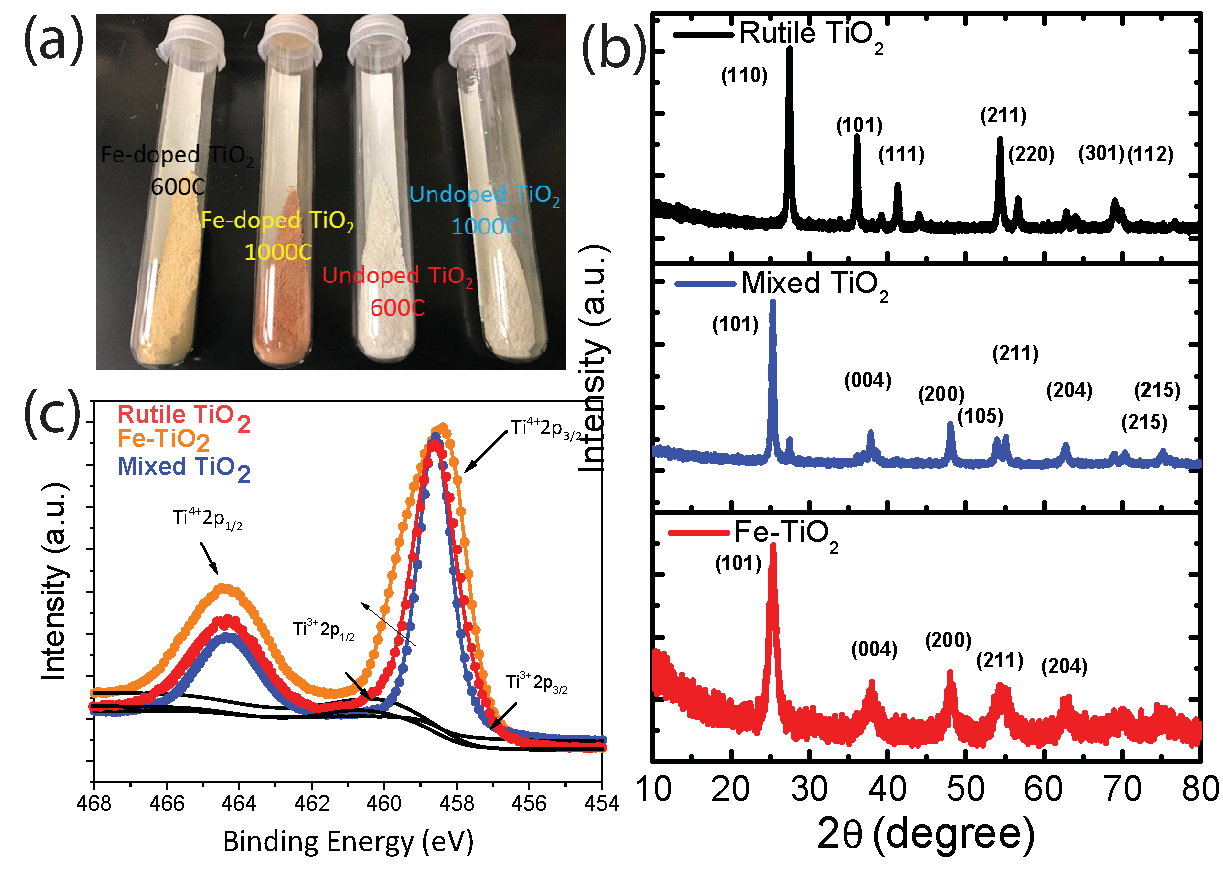
\includegraphics[width=0.45\textwidth]{scripts/figures/Materials}}
\caption{(a)Metal-doped Titania synthesized by sol-gel processing. (b and c) Material properties (crystallinty) and surface structure obtained from XRD and XPS.}
\label{fig:material}
\vspace{-2mm}
\end{wrapfigure}Oxide based materials have been heavily investigated as photocatalyst for both solar fuel production (hydrogen) as well as for water treatment\cite{tran_2012,lee_2016,nakata_2012}. The most abundantly studied oxide is titanium dioxide (\TIO). \TIO\hspace{2mm} is a wide band gap (3.2 eV), and therefore only absorbs UV light.  The PI has extensively synthesized and characterization \TIO\hspace{1mm} and metal doped \TIO\hspace{1mm} for photocatalytic nitrogen fixation (Fig. \ref{fig:material} and Fig. \ref{fig:experiments}). Characterizating the crystal structure and surface properties is accomplished through standard x-ray based and photo(electro)chemical characterization methods available to the PI at Georgia Tech (See Facilities). XRD provides insight into the crystal polymorphs (Fig. \ref{fig:material}b) and XPS provides quantative insight into the degree of defects (vacanies) at the surface (Fig. \ref{fig:material}c). In addition, rotating ring disk electrode experiments (Fig. \ref{fig:material}d) provides insight into the redox-based catalytic behavior of the minerals. 

Thus, the goal of this thrust is to synthesize nanoparticle-based oxides with controlled compositions. This includes oxides with various phases (anatase, rutile, brookite), size, and with different facets. Catalytic activity of oxides is well known to be dependent on the concentration of active sites, and all thus by tuning the various material properties we aim to identify what properties promote activity for various reactions (e.g. nitrogen fixation, denitrification, nitrification).  Considering the diverse nature of soils and sands, we also aim to epxlore additional oxides such as, iron oxides (FeTiO$_3$, Fe$_2$O$_3$, FeOOH), zinc oxide (ZnO$_2$), Tungsten trioxide (WO$_3$), and strontium titanate (SrTiO$_3$). These oxides were chosen based on their abundance in soils and sands (iron oxides) and their catalytic properties (ZnO$_2$,SrTiO$_3$,WO$_3$). Each mineral differs in terms of their electronic properties (bandgap and band edge locations), crystal structure and phase (anatase, rutile, brookite), crystal size, surface structuring (edge facets). In thrust I the PI will synthesize and characterize (experimentally and theoretically) the catalytic and electronic properties of these material prior their testing in thrust II and III.





\begin{comment}
\begin{wrapfigure}{r}{0.65\textwidth}
\centering
\vspace{-6mm}
\includegraphics[width=0.65\textwidth]{scripts/figures/PreliminaryData1}
\caption{Comparison of free energy pathways over pristine (blue), iron-doped (red) and oxygen-vacancy defect (black) for the associative (a) and dissociative (b) nitrogen reduction pathways at the equilibrium potential (adapted from Ref. \citenum{Comer_2017}). Titania and iron doped titania (c) and preliminary photocatalytic measurements (d).}
\label{fig:DFT_fixation_energies}
\vspace{-2mm}
\end{wrapfigure}
\end{comment}



\vspace{1mm}
\subsubsection{Synthesize oxide a nanominerals with controlled phase, facets and size}
\label{sec:SA1_1}
\vspace{1mm}

There have been no systematic investigations of the activity of mineral crystallinity on photocatalytic generation of \NO\hspace{1mm} and \NH. In addition, little work has been completed to evaluate the effect of particle size and shape (controlled facet). While large particles result in smaller effective surface area, these particles may have a higher concentration of bulk or surface defects which could promote various N-based transformations. In addition, surface structuring is critical to promote various intermediate processes (e.g. N-N and N-O activation), yet it is unknown what facets promote small nitrogen-based molecule activation. This objective seeks to conclusively define the active mineral phase and facet by evaluating the  turnover frequencies and quantum efficiencies.

The goal will be achieved by testing commercial oxides (e.g. Degussa P25), single crystals (e.g.TiO$_{2}$ (100), (101), Fe$_2$O$_3$ (0001), SrTiO$_3$ (100), SrTiO$_3$ (110), SrTiO$_3$ (111), ZnO (0001)), synthesized nanoparticles, and thin films under various reaction conditions. The synthesized oxide \begin{wrapfigure}{l}{0.5\textwidth}
\centering
\vspace{-12pt}
\fbox{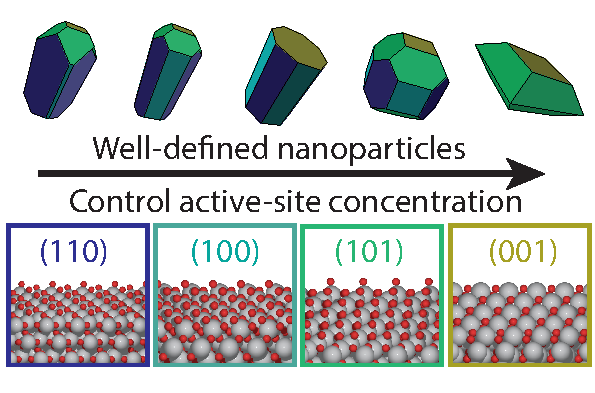
\includegraphics[width=0.5\textwidth]{scripts/figures/TiO2_facets}}
\caption{Well-defined nanoparticles will provide a route to control the relative concentration of various surface terminations for oxide based photocatalyst. Upper panels illustrate potential nanoparticle shapes while lower panels show low-energy surface terminations.}\label{fig:TiO2_facets}
\vspace{-14pt}
\end{wrapfigure}nanoparticles will have be be prepared primarily through wet chemical routes. Iron oxides can be synthesized through co-precipitating Fe$^{2+}$ and Fe$^{3+}$ aqueous salt solutions by the addition of base. Through varying the electrolyte chemistry (salts, pH, and ionic strength), the size, shape and composition of the nanoparticles can be tuned\cite{gupta_2005}. Titania and ZnO$_2$ will be prepared through standard sol-gel processing, and the material composition will be tuned through post processing methods (hydrothermal and thermal processing)\cite{chen_2009}. Again tuning the solution ionic strength and pH allows for the production of uniform size particles. SrTiO$_3$ will be made through a solid-state reaction conducted under microwave heating. Post-synthesis ball-milling will be required to attain particles at the nanoscale\cite{makarova_2010}. Finally, particles with controlled surface facets (TiO$_2$ and ZnO$_2$) will be generated through the use of capping or
surfactant based approaches during hydrothermal synthesis \cite{Dinh2009,Liao2007} (Figure \ref{fig:TiO2_facets}). Surfactants serve to limit the particle size, while capping approaches will be utilized to tune the growth direction. Amorphous nanoparticles of  can be synthesized using common sol-gel  \cite{ReyesCoronado2008}.  The vast array of commercial, single crystal and synthesized particles will enable us to decouple the role electronic and surface properties play in the evolution of \NH\hspace{1mm} and \NO\hspace{1mm} in thrust II and III. 



\vspace{1mm}
\subsubsection{Ex-situ Mineral Characterization}
\vspace{1mm}
Particles will be thoroughly characterized with microscopy (SEM/TEM) and
dynamic light scattering (DLS) to confirm the morphology, structure,
size uniformity and facets. Diffraction (XRD) approaches will be
utilized to confirm the phase and purity, and \NN{} physisorption be conducted on
nanoparticles to confirm the surface area. The thermal behavior, surface structure and surface chemistry of all synthesized catalyst will be characterized by differential thermal analysis (DTA), XRD and XPS. The presence of the Fe dopant should be visible through the thermic effects (curve shifting) and weight loss observed through the DTA analysis, as well as through inductively coupled plasma mass spectroscopy (ICP-MS) \cite{Huang_2001}.  In addition, the O1s, Ti2p, and Fe2p binding energies will be recorded using XPS to measure the oxidation states of Ti and Fe based surface species. Finally, UV/Vis spectroscopy
will be utilized to characterize the absorption and optical bandgap
changes that result due to from various synthesis approaches.



\vspace{1mm}
\subsubsection{Use ab-initio thermodynamics to compute surface coverages}
\vspace{1mm}
The preliminary results shown in Fig. \ref{fig:phase_diagrams} illustrate how DFT calculations can provide insight into the role of the environment on catalytic activity. This type of ab initio thermodynamic analysis will be extended to include the most promising materials and surface facets identified in Sec. \ref{sec:SA1}. The analysis will be extended to include a more diverse range of intermediates, including the oxidized/reduced nitrogen intermediates that form the reaction network for nitrogen fixation and nitrification. Furthermore, the analysis will be extended to include additional chemical potential variables, ultimately seeking to map out the most abundant surface species as a function of oxygen (O$_2$), hydrogen (H$_2$O), nitrogen (N$_2$) and carbon (CO$_2$). This high-dimensional map can be projected onto an arbitrary reaction condition so that the surface state can be analyzed in terms of temperature and gas ratios; Medford has demonstrated this technique in prior work on carbide and oxide surfaces under\begin{wrapfigure}{r}{0.5\textwidth}
\centering
\vspace{-1mm}
\fbox{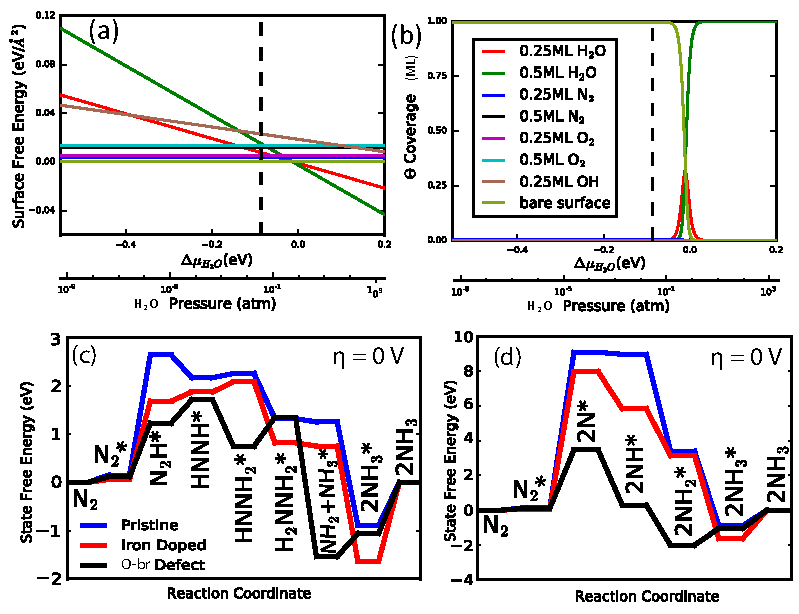
\includegraphics[width=0.5\textwidth]{scripts/figures/Theory}}
\caption{Surface free energy (a), coverage (b)for H$_2$O, N$_2$, O$_2$, and OH as a function of H$_2$O chemical potential. The relevant water potential under gas-phase conditions at 100\% RH (0.035 atm) is shown by dashed lines in (a-c). See Ref. \citenum{Comer_2017} for details.}
\label{fig:theory}
\vspace{-2mm}
\end{wrapfigure}  reaction conditions \cite{Medford_2012b, Medford_2014b}.

\vspace{1mm}
\subsubsection{Calculate interaction between different facets and probe molecules}
\vspace{1mm}The use of DFT provides significant insight into the energetics of binding of intermediates and various materials surfaces, as shown in Fig. \ref{fig:DFT_fixation_energies}. However, probing the full reaction network for nitrogen fixation and nitrification on the various surface facets of rutile, anatase, and hematite would be prohibitively expensive. In order to address this challenge we will select model surfaces for each material. These surfaces will be chosen based on stability (e.g. low-index facets such as rutile (110)) and hypothesized activity (e.g. oxygen vacancies and edge defects). We will select 3 representative surfaces for each material, as well as 6 surfaces that include both Ti and Fe to assess the effects of doping and chemical mixtures (e.g. Fe-substitution on rutile, Ti substitution on hematite), leading to a total of 15 model surfaces. In order to quickly screen these surfaces for nitrogen transformation activity we will utilize four probe molecules: N$_2$*, N*, NH*, and NO*. he binding energies of these probe molecules will provide insight into the reactivity of various 
surfaces toward dinitrogen as well as oxidized/reduced nitrogen species. The findings will be used, along with insight gained from experimental investigations, to identify the most reactive surfaces and to suggest other surfaces not in the original test set that might be more relevant. This iterative process will lead to computational models of the active site/surface on rutile, anatase, hematite, and mixtures of titania and hematite.
\vspace{1mm}

\subsubsection{Calculate free energy diagrams}
\label{sec:SA3_3}
\vspace{1mm}

The energetics of all relevant reaction intermediates for nitrogen fixation and nitrification will be computed for the surfaces with the most promising energetics (Sec. \ref{sec:SA1}) and the highest relative reactivity toward nitrogen species under relevant conditions (Sec. \ref{sec:SA2}). These energies will be used to generate free energy diagrams, similar to Figs. \ref{fig:DFT_fixation_energies} and \ref{fig:FEDs}. The CHE model will be used to assess the feasibility of reaction pathways under illumination, similar to Fig. \ref{fig:FEDs}b. Uncertainty quantification via the BEEF-vdW functional will provide estimates of the error due to the XC approximation, as illustrated in Fig. \ref{fig:FEDs}. This error estimate will allow efficient identification of the mechanisms that are most probable, while dismissing mechanisms that are thermodynamically infeasible. As the most likely mechanisms and active sites are identified they will be refined by inclusion of explicit solvent layers and use of higher-order theoretical methods such as DFT+U and HSE06. These calculations, coupled with the experimental characterizations, will result in a molecular-scale understanding of the active site and reaction mechanism of photon-driven nitrogen fixation and nitrification on anatase, rutile, and hematite surfaces.
\vspace{1mm}

\begin{comment}
Establishing a benchmark system for photoelectrochemical testing will be
of particular importance since these experiments have not been
previously reported. Various conductive supports (graphite, FTO, ITO, etc.)
will be utilized during testing depending on how the films will be
characterized and tested (spectroscopy, photoelectrochemical,
microscopy). Films will be tested, and the influence of particle size. Electrochemical impedance
spectroscopy (EIS) will be performed on thin films to measure the charge
transfer resistance of the photoelectrodes and catalysts. Catalytic
activity of the samples will be probed through varying the applied bias
with a potentiostat using a three electrode electrochemical cell, and quantum efficiencies will be obtained by
varying the photon energy through in situ UV/Vis spectroscopy.
Measured activity will be correlated with the relative abundance of
exposed facets to provide insight into which facets are
responsible for selective photo-catalytic nitrogen fixation\cite{Cargnello_2016}.
\end{comment}


%\subsubsection{Laboratory-based atmospheric incubation experiments}
%\vspace{2mm}

\newpage
\subsection{Thrust II: Impact of Soil properties}
\label{sec:SA3}
\vspace{1mm}
\subsubsection*{Introduction \& Preliminary Results}
\vspace{1mm}
\begin{wrapfigure}{r}{0.43\textwidth}
\centering
\vspace{-1mm}
\fbox{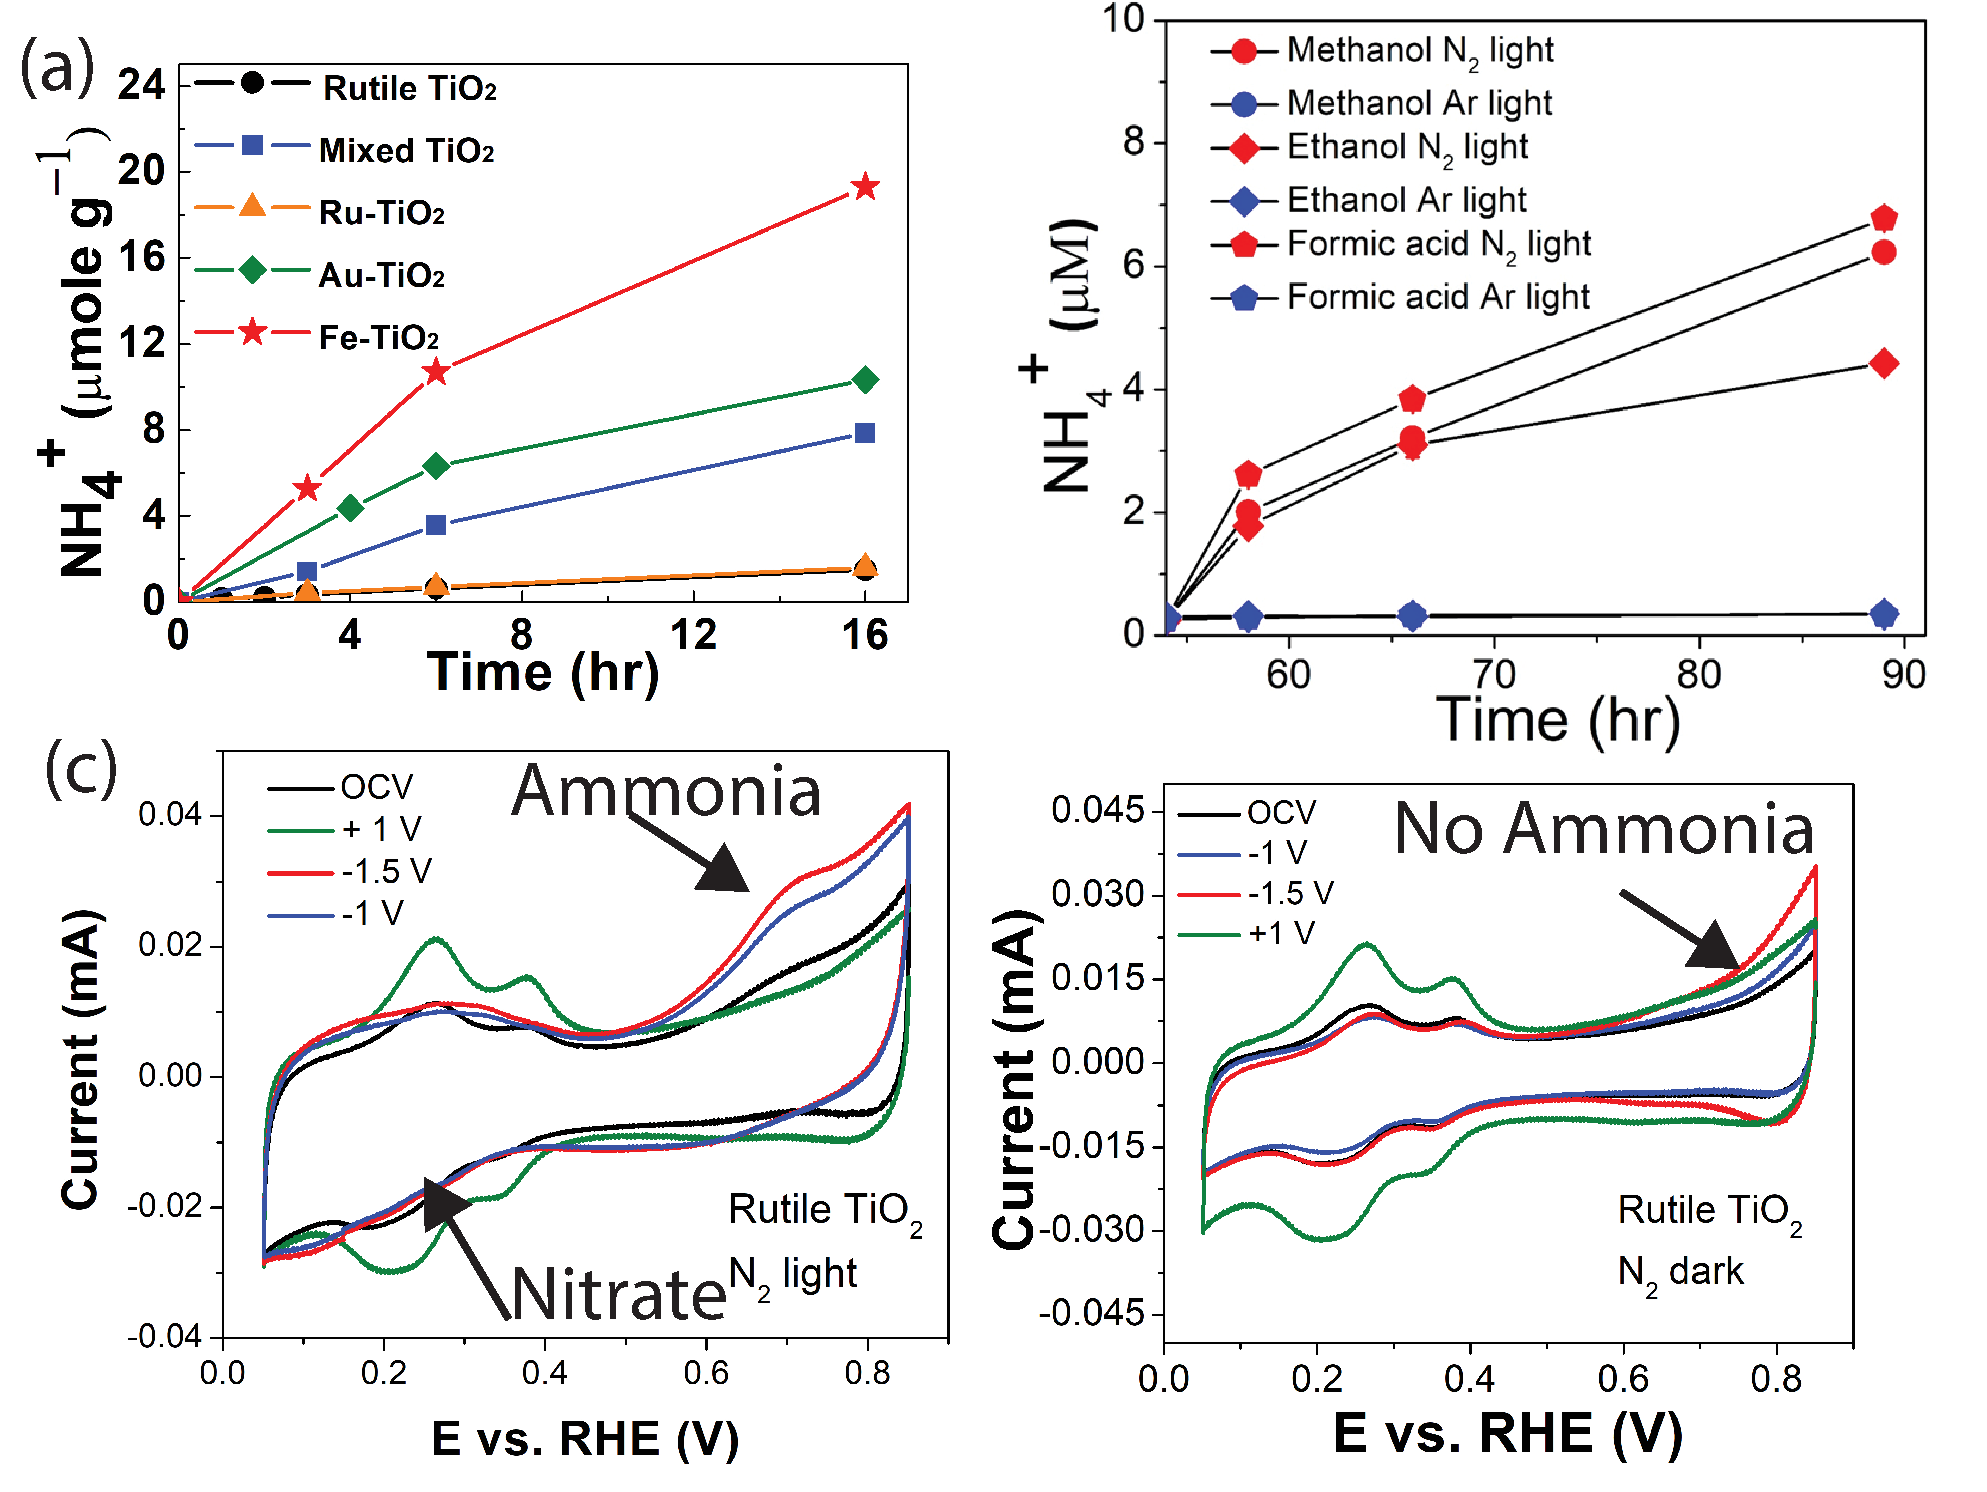
\includegraphics[width=0.43\textwidth]{scripts/figures/experiments}}
\caption{Photocatalysis experiments on metal doped TiO$_2$ (a) and TiO$_2$ with organic matter (b). Photocatalyzed nitrogen-based redox species on TiO$_2$ using rotating ring disk electrode experiments (c and d). }
\label{fig:experiments}
\vspace{-2mm}
\end{wrapfigure}Catalytic studies of nanoparticles and thin films with well-defined ratios of active facets have proven successful in elucidation and engineering of the active surfaces of titania for photocatalytic methanol decomposition \cite{Bennett_2016,Cargnello_2016}, and a similar strategy is expected to apply to nitrogen photofixation, photonitrification, and photodenitrification.  Initial experiments by the Hatzell lab have successfully reproduced early work completed by Shrauzer and Guth which focuses on understanding photofixation of nitrogen\cite{Schrauzer1977}. Titania catalysts synthesized using sol gel synthesis resulted in materials with optically visible differences (Fig. \ref{fig:material}a), which resulted in differences in the rate of photofixation of nitrogen with metal dopants (Fig. \ref{fig:experiments}a) and with organic matter present (Fig. \ref{fig:experiments}b). Overall, the results conclusively showed that ammonia is produced during photofixation on titania based minerals, and that the rate at which ammonia is produced increases in the presence of iron dopant. The role of the iron dopant has not yet been discerned, as it could aid in trapping electrons, activating nitrogen or may promote various defects (oxygen vacancies). Despite this, the initial experiments support the findings that photofixation of nitrogen is possible on titania and iron-doped titania. 




%The nitrogen fixation, nitrification and denitification activity of these nanoparticles and thin films will be tested for photocatalytic activity under humidified or dry gas. The performance will be benchmarked with isotopically labeled nitrogen to avoid issues of contamination, and products formed will be evaluated through traditional means (GC/MS/NMR).
\vspace{1mm}
\subsubsection{Evaluation of the impact soil pH}
\vspace{1mm}


\vspace{1mm}
\subsubsection{Impact of Soil Moisture Content}
\vspace{1mm}

\vspace{1mm}
\subsubsection{Evaluation of the impact of Fertilizer (NH$_3$ Concentration)}
\vspace{1mm}


\vspace{1mm}
\subsubsection{Electrochemical Characterization of Redox Processes}
All synthesized catalyst will be evaluated for their redox behaviour using a rotating ring disk electrode (RRDE) system. A thin film of the particles will be dispersed on a graphite electrode which is rotated at various speeds in an electrolyte. Through baising (electrochemical) the ring electrode while the disk is not biased the redox behaviour of the various intermediates formed during the photocataytic tests can be discerned. Specific nitrogen based gases and compounds can  (e.g. nitrate, nitrite, NO, N$_2$, NH$_3$) will be dissolved or saturated in the electrolyte and the redox peak will be discerned in a controlled environment. Correlating the observed peaks with the control peaks can provide insight into what dominate reactions are occurring on the various minerals as a function of their size, shape, structure. 


%Furthermore, DFT-based computational studies have provided initial insight into the thermodynamics of nitrogen fixation on rutile (110) and iron-doped rutile (110) surfaces. The free energy pathway for dissociative (i.e. direct N-N bond scission) and associative (i.e. N$_2$ hydrogenation before dissociation) mechanisms on pristine rutile (110), an oxygen O-br vacancy on rutile (110), and an Fe-substitution on rutile (110) are illustrated in Fig. \ref{fig:DFT_fixation_energies}. The results indicate that Fe surface sites do not significantly improve the energetics, while the presence of O-br vacancies significantly improves the binding of NH$_x$ species. However, the low stability of N* and HNNH* result in thermodynamic barriers of $>$ 1.5 eV that are not surmountable at room temperature. Thus, the question of how the N-N bond is dissociated on TiO$_2$ remains an open question. In the same work\cite{Comer_2017}, we show that oxidative N-N bond scission is more favorable, and that the pathway for photo-nitrification on TiO$_2$ is thermodynamically feasible under illumination. This suggests that a complex interplay of photocatalytic reductive and oxidative processes governs the interaction between TiO$_2$ and nitrogen species. However, significant work remains to understand the role of other rutile facets and surface defects, and the energetics of nitrogen fixation and nitrification on both anatase and hematite.




\begin{comment}
\begin{wrapfigure}{r}{0.33\textwidth}
\centering
\vspace{-1mm}
\fbox{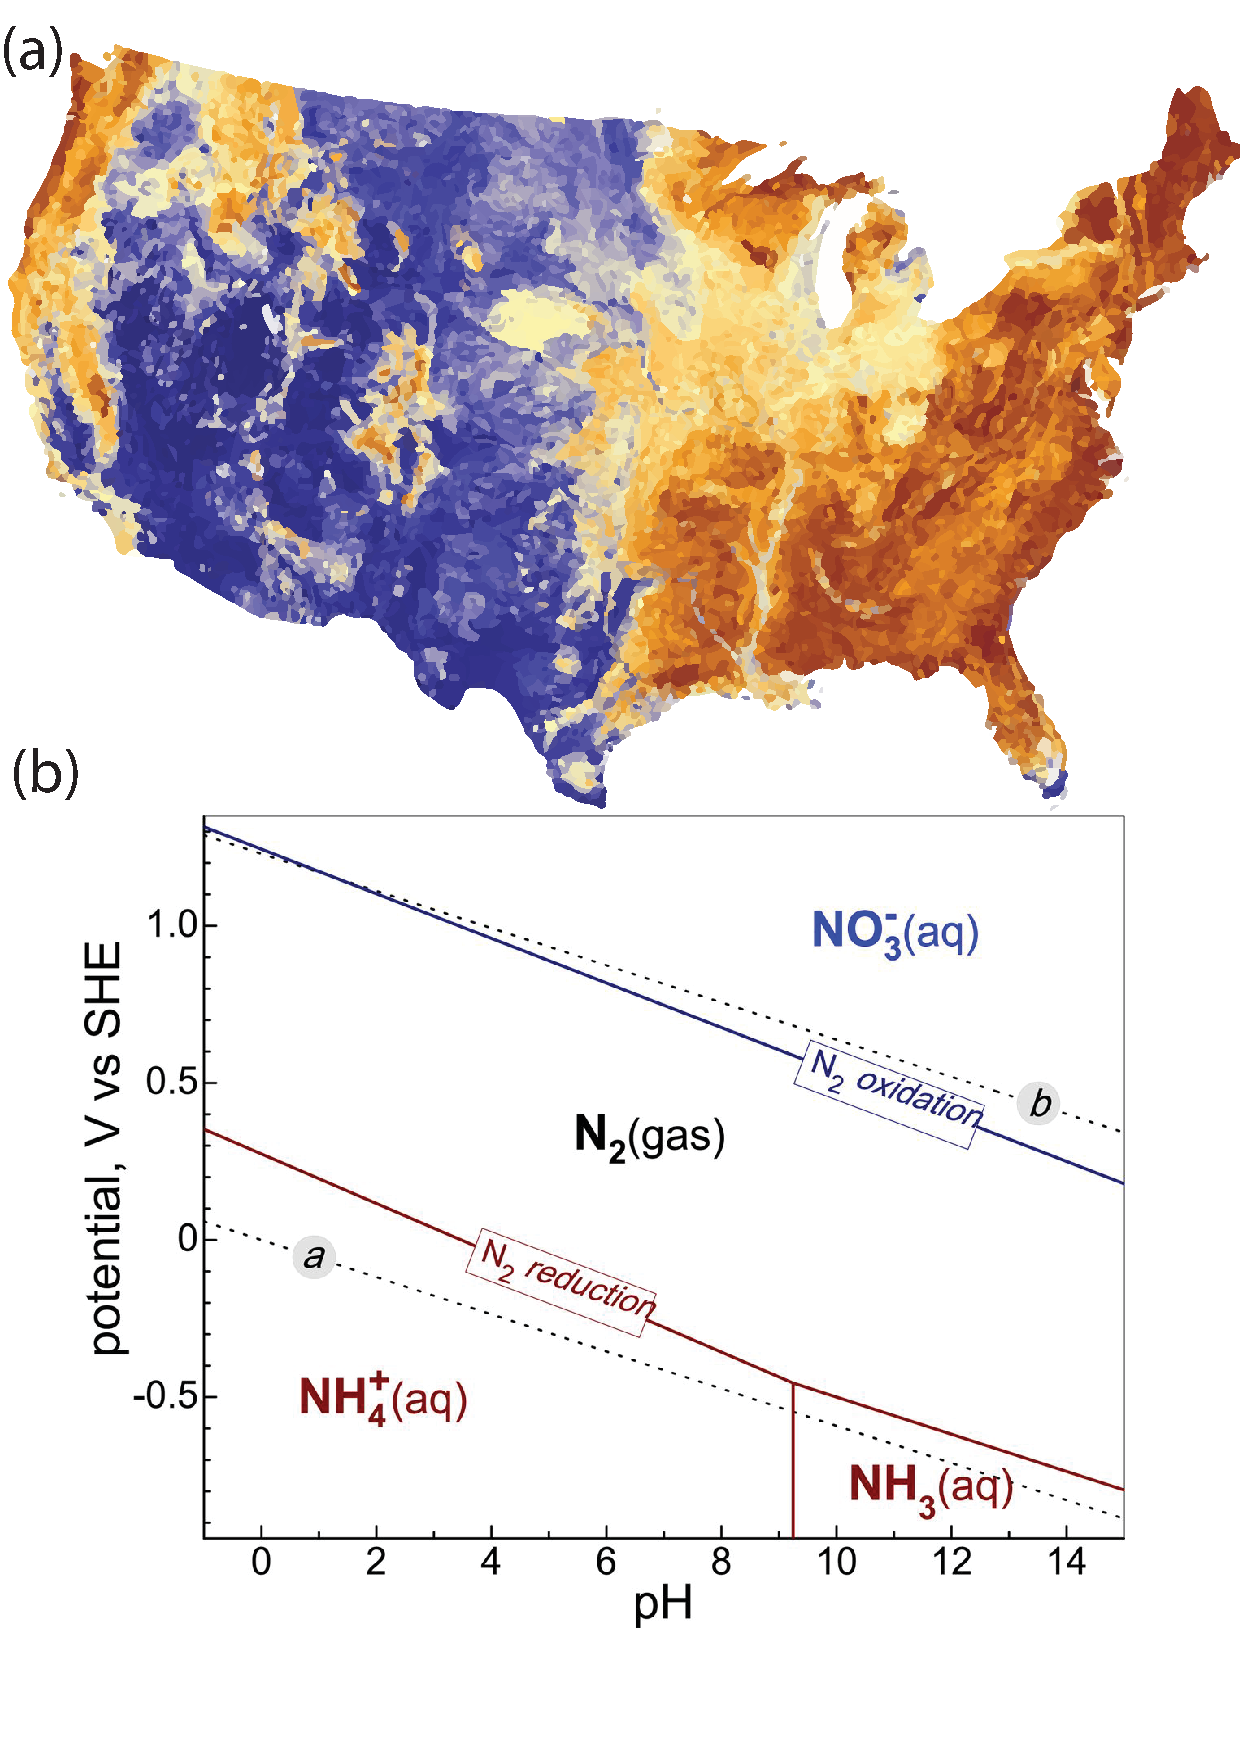
\includegraphics[width=0.33\textwidth]{scripts/figures/Acid}}
\caption{}
\label{fig:acid}
\vspace{-2mm}
\end{wrapfigure}
\end{comment}

\newpage
\subsection{Thrust III: The role of atmospheric properties on photocatalyzed N\textsubscript{2}O and \NH }
\label{sec:SA3}
\vspace{2mm}

\subsubsection*{Introduction \& Preliminary Results}
\begin{comment}
\begin{wrapfigure}{r}{0.6\textwidth}
\centering
\vspace{-30pt}
\includegraphics[width=0.6\textwidth]{scripts/figures/XPS_Fig.pdf}
\caption{\label{fig:experiment3}(a) Ambient pressure XPS  at LBNL (b and C) corresponding C1s and N1s spectra revealing dark (red dot) and light (green dot) peaks and (e and f) corresponding C1s and N1s spectra revealing dark (red dot) and light (green dot) peaks. (d) Ambient pressure is attained using a differential pumping between the sample and analyzer.}
\vspace{-10pt}
\end{wrapfigure}
\end{comment}

\subsubsection{Impact of Solar Intensity}
\vspace{2mm}

\subsubsection{Impact of Gas Composition}
\vspace{2mm}


\subsubsection{Impact of Temperature}
\vspace{2mm}

%In-situ electron paramagnetic resonance (EPR) and Ultra-violet/Visible (UV/Vis) spectroscopy will be utilized to discern the photoactivity and trapping sites on the catalyst during photocatalysis. X-band EPR is exceptional at directly probing the electron trapping dynamics through controlled low temperature (helium cooled) experiments in the presence of hole scavengers. Through integration of EPR spectra, paramagnetic spin concentration can be determined during experiments. Interstitial concentrations of Ti3+ and Ti4+ can be estimated (g\~1.9), and hole trapping sites at the surface have been previously observed (g=2.014). Through variable temperature testing (10 K to 300 K), transient charge separation and recombination can also be monitored. Total electron concentration during EPR testing will be obtained with UV/Vis. Gaining insight into the total electron concentration can aid in providing quantitative information regarding the percentage of electrons which are become trapped during their transport to the conduction band. These results will aid in providing detailed molecular level information regarding carrier transport and during the photoexcited process, which will inform DFT calculations. 

%Transfer of holes from the valance band can occur if an electron donor adsorbs to the electrode surface. More commonly this is referred to as electron transfer from an adsorbate to the photo-generated hole in the valence band. Understanding the dynamics of these “hole transfer” processes has primarily been completed through the use of thiocyanate (SCN-) as a hole scavenger. Extensive experiments on TiO$_2$ have shown the electron transfer process from SCN- to the photo-generated hole may take place on the picosecond time scale, which is significantly faster than the rate of electron-hole recombination process. While the hole transfer process on TiO$_2$ is relatively efficient, a range of time scales have been reported for other hole accepting adsorbates (alcohols, diols, carbohydrates), lasting from picoseconds to hundreds of nanoseconds. This points to the adsorbate limiting the rate at which a photo-generated hole can be transferred, rather than the TiO$_2$. Hole scavengers (SCN-) will be used during the ultra-fast spectroscopy testing to evaluate if photoreduction of nitrogen to ammonia is possible with and without catalyst and dopants. 
%\vspace{2mm}



\begin{comment}
\newpage
\vspace{2mm}
\subsection{Thrust III:  The impact of soil \MakeLowercase{p}H and moisture content}
\vspace{2mm}

\label{sec:SA2}

\subsubsection*{Introduction \& Preliminary Results} 
\vspace{2mm}

Thrust III will leverage the materials synthesis (Thrust I) and testing (Thrust II) in order to provide \emph{fundamental insight into the nature of interactions between mineral surfaces and nitrogen species} under environmentally-relevant photocatalytic conditions. This thrust will make use of advanced in- and ex-situ spectroscopic techniques, including XPS, EXAFS, and EPS, in order to probe the interaction between mineral surfaces and adsorbed species. This will be coupled with DFT calculations of free energy pathways to unravel the complex phenomena that enable photocatalyic nitrogen transformations at the surfaces of titania and hematite materials. 

\begin{comment}
\begin{figure}[ht]
\centering
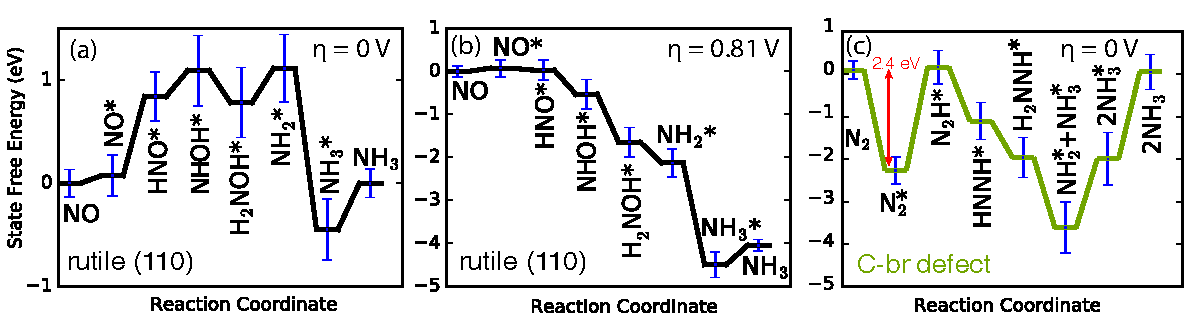
\includegraphics[width=\textwidth]{scripts/figures/nitrification_Cdefect_FED.pdf}
\linespread{1.0}
\vspace{-6mm}
\caption{Reaction free energy diagrams for reverse nitrification at rutile (110) at the equilibrium potential (a), and at a potential equivalent to the conduction band edge of TiO$_2$ (b) \cite{Comer_2017}, and free energy of nitrogen fixation at the C-br defect at the equilibrium potential (c). Error bars represent one standard deviation of the BEEF-vdW ensemble\cite{Wellendorff2012,Medford2014a}.}\label{fig:FEDs}
\end{figure}
\end{comment}

%Performing in situ surface science based experimentation allows us to begin to better understand the photofixation pathways. Typically, however, surface science measurements such as XPS require ultra high vacuum environments, which are not environmentally relevant. To begin to evaluate environmentally relevant conditions Hatzell has led efforts to perform in-situ experimentation at Lawrence Berkeley's Advanced Light Source. This facility has the unique capabilities of having near ambient pressure XPS (AP-XPS). We were the first researchers to begin to evaluate nitrogen photofixation using this technique when we traveled there in August 2017. Our preliminary trip allowed us to begin to evaluate single crystal titania, which was used as a model system to evaluate through theory. Single crystals are non-ideal substrates for photocatalysis as they have few defects, and therefore nitrogen activation is difficult. Future testing to be completed in December of 2017, will move toward evaluating amorphous semiconducting materials which will be discussed in detail below.

%Despite these challenges, our initial AP-XPS results have already provided unprecedented insight into nitrogen fixation at a rutile (110) surface, as well as opened new questions and hypotheses regarding the nature of the active site. In the initial experiments photofixation of nitrogen to a reduced form was detectable (Fig. \ref{fig:experiment3}c). This was observed through the change in the N1s spectra. No oxidized nitrogen species were detected in either the N1s or O1s peaks. Interestingly, the N1s peak which was responsive to light (corresponding to reduced nitrogen), was only responsive when trace amounts of amorphous carbon was on the titania. If this impurity was oxidized from the surface, the shifted N1s peak disappeared (Fig. \ref{fig:experiment3}b-f). These advanced surface science provides evidences that not only defects play a role, but environmental impurities (like carbon) also may be critical for photofixation. We intend to further investigate these impurities in Thrust III. 

%These results are complemented by DFT calculations of the free energy pathway of both nitrogen fixation (Fig. \ref{fig:DFT_fixation_energies} as well as reverse nitrification on the rutile (110) surface (Fig. \ref{fig:FEDs}a-b); however, these free energy diagrams suggest that formation of reduced nitrogen species is limited by thermodynamic barriers, although we note that reverse nitrification is thermodynamically feasible under photocatalytic conditions (Fig. \ref{fig:FEDs}b). This raises the question of how the N-N bond is dissociated on the rutile surface. While the question remains open, the insight regarding surface carbon species suggests a particularly promising hypothesis that surface carbon participates in photocatalytic nitrogen fixation. The energetics of a carbon substituted for a bridging oxygen (C-br) defect for nitrogen fixation is shown in Fig. \ref{fig:FEDs}(c). This reveals a remarkably strong N$_2$ binding energy of -2.4 eV, compared to an endergonic adsorption of 0.2 eV for N$_2$ on other rutile sites (Fig. \ref{fig:DFT_fixation_energies}). Although the subsequent hydrogenation to N$_2$H is highly exergonic, this computational finding supports the hypothesis that carbon may play a key role in the process. The goal of this thrust is to discern the nature of the active site and rate-liming step for various nitrogen transformations at titania and hematite surfaces.

\vspace{2mm}
\end{comment}

\subsection*{Risk Assessment \& Contingency Plan}
\label{sec:risks}
\vspace{2mm}

One potential risk is the possibility that the rate-limiting reaction occurs via a direct photo-excitation of an adsorbed complex. This will complicate experimental investigations, and  necessitate the use of an excited-state theoretical method that goes beyond DFT. Given the preliminary results, and modern understanding of the similar water-splitting process \cite{Hellman_2017}, we anticipate that this situation is unlikely; however, in the case that it occurs we will employ a two-pronged contingency plan. First, the proposed thermodynamic theoretical approach will still be useful in identifying the relevant initial state of the photo-excited rate-limiting reaction, and EPR experiments will aid in identifying charge transfer dynamics. Second, the GW approximation will by applied to the initial/final state complexes in order to assess the unoccupied states and excitation dynamics. This will provide insight into experimental investigations to probe specific photon absorption bands near the excitation frequency of the initial state. %<- not sure how good/bad of a "contingency plan" this is... it might just confuse them. Feel free to modify/remove. The main thing is probably to point out that we will use GW if excited state information is needed. Of course we should probably have some other experimental risks and alternate plans as well.

\vspace{2mm}
\subsection{Timeline \& Responsibilities}
\vspace{2mm}

\begin{wrapfigure}{r}{0.45\textwidth}
\vspace{-30pt}
\centering
\includegraphics[width=0.45\textwidth]{scripts/figures/Gantt.pdf}
\caption{\label{fig:Gantt} Timeline and Responsibilities}
\end{wrapfigure}

The project will  be carried out by 2 graduate students, one  advised by co-advised by Medford and Hatzell and one co-advised by Hatzell and Tang. The research questions will be pursued roughly sequentially, with significant overlap. Figure \ref{fig:Gantt} shows the proposed timeline for the task associated with each thrust. The PI's will share responsibility for the completion of all tasks, but each task will be led by a PI based on their core expertise. Hatzell will lead all photochemistry thrusts, Medford will lead all computational efforts, and Hatzell and Tang will divide the materials synthesis and characterization efforts. There will be close communication between the computational and experimental efforts, with bi-monthly meetings scheduled to aid in guiding both efforts in tandem. 
\vspace{2mm}

\section{Broader Impacts}
\label{sec:BI}
\vspace{2mm}

\subsection{Broader Impacts to Society}
\vspace{2mm}

Managing the nitrogen cycle has been deemed a critical component of the food-energy-water (FEW) nexus, as control over the composition of reduced and oxidized nitrogen species in soils is needed for adequate food production. Furthermore, with growing populations in a range of centralized and decentralized regions, understanding nutrient transformations processes will only grow in importance. The critical first step in managing the nitrogen cycle, will only come if the magnitude and mechanisms of each N-based transformation is defined. This is historically difficult, as the  nitrogen cycle is known to be the most complex biogeochemical nutrient cycle.  The proposed broader impact of this work will specifically aim to determine how solar-driven abiotic N-transformations contribute to nutrient cycles. The resulting fundamental insights will enable prediction of how environmental factors affect nitrogen transformation rates, providing key inputs into advanced quantitative models of the nitrogen cycle. Furthermore, the insight from this work has implications for the development of new technologies distributed fertilizer production via fixing nitrogen at ambient conditions, as well as potential new routes to mitigate nitrate pollution in groundwater.

\vspace{2mm}

\subsection{Education and Outreach}
\vspace{2mm}

\subsubsection*{Advance discovery and understanding while promoting teaching, training, and learning:} Georgia Tech is currently launching a 10 year program aimed at better incorporating the ideas surrounding social sustainability into the curriculum and student body. This program is called ‘Serve-Learn-Sustain’ (SLS). Hatzell and Tang served as a Food-Energy-Water (FEW) fellows within the program, and Medford is currently an Energy Fellow. The aim of this program is to bring together faculty, to discuss ways to incorporate the ideas from their research (Abiotic Nitrogen Cycle), into their courses. The PIs are each currently applying various relevant aspects of this project into their courses (thermodynamics, numerical methods, geochemistry). 

In addition, through an internal competition, Hatzell and Medford raised funds to support a food-energy-water related capstone project for Georgia Tech Seniors. Specifically, the PI's are designing a capstone 2018 semester which will have the students focus their efforts on building a small scale dinitrogen photofixation reactor and analyze the fertilization capacity of the resulting effluent. The capstone will be multi-disciplinary, and will have aspects related to technological development as well as social sustainability to align with the goals of the Serve-Learn-Sustain program. All PIs are also specifically working with the SLS program to \underline{\textbf{assess}} students connection to FEW related topics. A survey will be collected in each class at the beginning and the end of the semester to assess how students' views evolved on FEW related topics.
\vspace{2mm}

\subsubsection*{\textbf{Enhancing Infrastructure for Research and Education}}
\vspace{2mm}

The PIs aim to enhance the infrastructure of ambient pressure XPS for photocatalysis by collaborating with staff scientists at national labs to build research and education networks for the participating students. Specifically the PI's aim to work with Ethan Crumlin at Lawrence Berkeley National lab (LBNL), to perform in situ surface science measurements using AP-XPS. The infrastructure developed to apply AP-XPS to measure nitrogen species at mineral surfaces will also have relevance for numerous other systems in the emerging field of photo(electro)chemical nitrogen chemistry.

\vspace{2mm}

\subsubsection*{\textbf{Broadening dissemination to enhance scientific and technological understanding}}
\vspace{2mm}

Due to the fact that this is a relatively new field of study with tangible implications the PI's will maintain a publicly accessible website detailing our findings and contribute to relevant Wikipedia articles\cite{wiki_photogeochemistry}. Graduate students working on the project will create YouTube videos which describe experimental and theoretical approaches taken during the research program. The fact that the proposed research deals with ambient conditions and common materials leads to a low barrier for interested citizens to conduct simple experiments that are reported in the videos. Disseminating the findings in an open access fashion will aid in accelerating the rate of other researcher's work and engaging public interest. 
\vspace{2mm}

\subsubsection*{\textbf{Broadening the participation of underrepresented groups}}
\vspace{2mm}

The PIs have a history of recruiting underrepresented and minority students. All PIs will apply for REU support to not only support graduate students but undergraduates on this project, with a particular emphasis on recruiting underrepresented minorities. Medford supports the Summer Undergraduate Research Exchange (SURE) and Exxon Mobil ChBE Steps programs at Georgia Tech that allow underrepresented minority students to work on research projects during the summer. The Steps program is specifically targeted to universities with a large number of underrepresented minority students and attempts pave the way for them to obtain a dual degree from their original university and Georgia Tech. 

\vspace{2mm}
\section{Results from Prior NSF Support}
\vspace{2mm}
\textbf{Hatzell}: CBET-1706290 Collaborative Research: EPRI/WERF: Collaborative Research: Electrical percolation in flowable electrodes for energy-efficient water re-use applications, (Marta Hatzell: \$69,245.00 , 08/15/17- 07/31/18). \textbf{Intellectual Merit:} This project seeks an improved understanding of the electrical and ionic percolation in flow electrodes. The work aims to evaluate flow electrode structure using X-ray Tomography and to correlate the fractal structuring to system performance. \textbf{Broader Impacts:} In addition to advancing water treatment technology science, the impacts of this grant include participation from the Georgia Intern for Teachers (GIFT) program. The PI had two high school teachers join her group to begin to integrate the scientific findings into a a high school science curriculum. \textbf{Publications:} Two papers from this project was published \cite{zhang2017combined,2017Hatzell}another two papers are in preparation.
\\ \noindent

\\ \noindent
\textbf{Medford} has been awarded \textit{SusChEM: Collaborative Research: Surface Reaction of Oxygenates on Lewis Acidic Metal Oxides} (CBET 1705444, \$300,000, 8/1/2017 - 7/31/2020). \textbf{Intellectual Merit:} This project focuses on understanding how elementary reactions for sugar conversion are affected by electronic properties and geometric factors of oxide surfaces. \textbf{Broader Impact:} The project will focus on recruiting underrepresented graduate and undergraduate students through the STEP program at Georgia Tech, and will enhance student training by allowing students to work in diverse scientific environments. This project has not yet started so there are no relevant products.
\setcounter{page}{1}
\renewcommand{\LeftFooter}{References}
\renewcommand{\PageLimit}{0} %0 page limit puts no "of X" in page numbers

\bibliography{references}
\bibliographystyle{unsrt-noetal}
\setcounter{page}{1}
\renewcommand{\LeftFooter}{Data Management Plan}
\renewcommand{\PageLimit}{2}

\begin{center}
{\bf Data Management Plan} \\*[3mm]
\end{center}

\setcounter{section}{0}

\section{Overview}
The data management plan (DMP) is for the project ``\@title''. The plan requires no additional cost, as data are stored on the computer where the data originated, backed up to a central server specifically meant for data storage and sharing amongst PI’s, and ultimately disseminated through publications and open databases that are free to the public.

\section{Capture}
\subsection{Experimental data}
The characterization and testing of catalytic samples will lead to data of the following types: gas chromatography traces, infrared and ultraviolet-visible spectra, X-ray photolectron spectra, X-ray absorption spectra, X-ray diffraction patterns, nitrogen physisorption isotherms, elemental analysis reports, transmission and scanning electron micrographs, EDS and EELS maps, mass spectrometry data, temperature programmed desorption data. The data is typically obtained as an output file from the software that operates an instrument. In some cases, files will be received from collaborators or commercial service laboratories. In order to facilitate collaboration amongst the PI’s these files will be periodically transferred to a central server in the PACE supercomputing cluster.

\subsection{Computational data}
Data generated by computational simulations will automatically be captured on the PACE cluster.

\subsection{Metadata}
Capture and storage of metadata is critical to ensure the reproducibility and long-term value of the data. Both experimental and computational data will have associated meta-data. The experimental metadata will mainly consist of experimental details of catalyst preparation, reaction procedures, and characterization procedures, while computational meta-data will consist of the necessary inputs and scripts to reproduce the data. The metadata will be initially captured in standard or electronic laboratory notebooks, and transferred to a standard digital format (json) when the data is transferred to the central server. The json files containing pertinent metadata will be permanently stored with the raw data.

\subsection{Physical samples}
Samples will be stored and catalogued according to established procedures in the Hatzell group. The standardized format will enable data retrieval by project, date, or conditions. Samples typically do not have an indefinite shelf life, and will be disposed 5 years after the project ends.

\section{Analysis}
Data analysis is critical to extracting useful knowledge from raw data. For this project, the raw experimental data will be processed to determine various characteristics of catalysts, such as surface areas, dispersions of supported species, and the nature and concentration of surface species, and raw computational data will be analyzed to determine key quantities such as surface, adsorption, and activation energies, charge distributions, and band gaps. Some analysis workflows are standardized and included in commercially available software packages, while others are customized and evolving. When standardized analysis techniques are used this will be included as metadata and stored with the results of the analysis. Customized workflows will also be captured by storing the necessary scripts along with the analysis results.

\section{Sharing and Dissemination}

\subsection{Data Sharing}
Sharing data, metadata, and analysis workflows amongst the Hatzell, Tang, and Medford groups will enable efficient collaboration. A central server within the PACE cluster will be used to facilitate easy access to shared data, and metadata capture will ensure that shared data has the necessary context to be useful. Furthermore, the MATIN e-Collaboration platform currently under development at Georgia Tech will be explored as a route to share intermediate results, workflows, and discussions via “research blogs”. These blogs will initially be private to ensure data security, but can easily be opened to the public once results have been published.

\subsection{Data Sharing and Dissemination}
The broad dissemination of research data as fundamental to progress in science. As such, published data generated within this proposal will be made freely and publicly available in compliance with the data sharing directive issued by the Office of Science and Technology Policy and relevant funding agencies. Specifically, publishable data and associated metadata will be uploaded to Citrination, the web-based data platform for materials, chemical, and device information. Citrine Informatics will host these data at no cost to this contract, or the government, for public access. In addition, computational reaction energies/barriers will be uploaded to the CatApp platform for broad dissemination within the computational catalysis community. Data shared will include: experimental procedures, material characterization, analysis of surface reactions, performance of catalysts, and adsorption/activation energies.  Data will also be available through journal publications – either the article or the supplemental information - and completed theses.


\section{Preservation}
\subsection{Storage and Backup during the Project}
Data will be stored locally on the computer of the data origination and will be periodically transferred securely over the campus network to a central server for longer-term data retention. Similarly, data from experiments at national laboratories will be copied onto a USB drive at the end of a trip and transferred to the server at GT. The fact that the central server will be used to share data amongst the PI’s will ensure that relevant data is transferred to the server at an appropriate frequency. The network server is a dedicated server that is backed up automatically. The data on the server is preserved for at least a period of seven (7) years where it is locally accessible, and then the data is preserved offline for three (3) more years, accessible with assistance from local network specialists. 

\subsection{Data Storage Duration} Digital data and metadata will be retained for ten (10) years on the centralized server. Physical laboratory notebooks will be stored by each faculty advisor for at least five (5) years. The most critical data will be widely disseminated, ensuring that it is available through publication outlets and open databases on a permanent basis.

\section{Protection}
All unpublished data will be stored on computers within secure campus networks. At this time, no additional security elements should be required.

\section{Rationale}
Georgia Tech commits to provide server space for the results from the proposed work for at least 10 years. The costs are covered as part of the requested indirect costs. The use of publication outlets and open databases provides a cost-effective approach to ensure that the most critical data are available on a permanent basis.

\setcounter{page}{1}
\renewcommand{\LeftFooter}{Biosketch}
\renewcommand{\LeftHeader}{Andrew J. Medford}
\renewcommand{\PageLimit}{2}
\begin{center}
{\bf Andrew J. Medford Biosketch} \\*[3mm]
\end{center}
\setcounter{section}{0}
\section{Professional Preparation}\label{AJM-professional-preparation}

\begin{itemize}
\itemsep1pt\parskip0pt\parsep0pt
\item
  North Carolina State University Raleigh, North Carolina

  \begin{itemize}
  \itemsep1pt\parskip0pt\parsep0pt
  \item
    B.S., Textile Engineering, 2009
  \end{itemize}
\item
  Stanford University, Stanford, California

  \begin{itemize}
  \itemsep1pt\parskip0pt\parsep0pt
  \item
    Ph.D, Chemical Engineering, 2015
  \end{itemize}
\item
  Georgia Institute of Technology, Atlanta, Georgia

  \begin{itemize}
  \itemsep1pt\parskip0pt\parsep0pt
  \item
    Postdoc, Mechanical Engineering, 2015-2016
  \end{itemize}
\end{itemize}

\section{Appointments}\label{AJM-appointments}

\begin{itemize}
\itemsep1pt\parskip0pt\parsep0pt
\item
  \emph{Assistant Professor - 01/01/2017-present}

  \begin{itemize}
  \itemsep1pt\parskip0pt\parsep0pt
  \item
    Georgia Institute of Technology, School of Chemical and Biomolecular
    Engineering
  \end{itemize}
\end{itemize}

\section{Products most closely related to the proposed
project:}
\def\labelenumi{\arabic{enumi}.}
\nobibliography*
\begin{enumerate}
\item \bibentry{Medford_2017}
\item \bibentry{Comer_2017}
\item \bibentry{Medford_2014a}
\item \bibentry{Vojvodic_2014}
\item \bibentry{Ulissi_2017}
\end{enumerate}

\section{Other significant products:}\label{AJM-other-significant-products}

\begin{enumerate}
\def\labelenumi{\arabic{enumi}.}
\item \bibentry{Medford_2015}
\item \bibentry{Medford_2015a}
\item \bibentry{Gomberg_2017}
\item \bibentry{Yang_2016}
\item \bibentry{Medford_2014b}

\end{enumerate}

\section{Synergistic Activities}\label{AJM-synergistic-activities}

\begin{enumerate}
\def\labelenumi{\arabic{enumi}.}
\item Currently lead `Big Data and Quantum Mechanics' vertically integrated project for undergraduate research on development of software at the intersection of machine learning and electronic structure theory.
\item Visited and hosted researchers from International Fertilizer Development Center (IFDC) to foster collaboration with Georgia Tech.
\item Participant in SLS Energy Systems for Sustainable Communities Fellows program in 2017.
\item Participant in ASEE Summer School for Chemical Engineering Faculty in 2017.
\item Member of grand-prize-winning team for AFRL ``Materials Data Science and Engineering Challenge'' in 2016.

\end{enumerate}
\setcounter{page}{1}

\renewcommand{\LeftFooter}{Biosketch}
\renewcommand{\LeftHeader}{Marta C. Hatzell}
\renewcommand{\PageLimit}{2}
\begin{center}
{\bf Marta C. Hatzell Biosketch} \\*[3mm]
\end{center}

\setcounter{section}{0}
\section{Professional Preparation}\label{MCH-professional-preparation}

\begin{itemize}
\itemsep1pt\parskip0pt\parsep0pt
\item
  Pennsylvania State University, University Park, Pennsylvania

  \begin{itemize}
  \itemsep1pt\parskip0pt\parsep0pt
  \item
    B.S., Mechanical Engineering, 2009
  \end{itemize}
\item
  Pennsylvania State University, University Park, Pennsylvania

  \begin{itemize}
  \itemsep1pt\parskip0pt\parsep0pt
  \item
    MS, Mechanical Engineering, 2010
  \end{itemize}
  \item
  Pennsylvania State University, University Park, Pennsylvania

  \begin{itemize}
  \itemsep1pt\parskip0pt\parsep0pt
  \item
    MS, Environmental Engineering, 2014
  \end{itemize}
\item
  Pennsylvania State University, University Park, Pennsylvania

  \begin{itemize}
  \itemsep1pt\parskip0pt\parsep0pt
  \item
    Ph.D, Mechanical Engineering, 2014
  \end{itemize}
\item
  University of Illinois, Urbana Champaign, Illinois

  \begin{itemize}
  \itemsep1pt\parskip0pt\parsep0pt
  \item
    Postdoc, Material Science and Engineering, 2014-2015
  \end{itemize}
\end{itemize}

\section{Appointments}\label{MCH-appointments}

\begin{itemize}
\itemsep1pt\parskip0pt\parsep0pt
\item
  \emph{Assistant Professor, 08/15/2015- Present}

  \begin{itemize}
  \itemsep1pt\parskip0pt\parsep0pt
  \item
    Georgia Institute of Technology, George W. Woodruff School of Mechanical Engineering
  \end{itemize}
\end{itemize}

\section{Products most closely related to the proposed
project:}\label{MCH-products-most-closely-related-to-the-proposed-project}

\begin{enumerate}
\def\labelenumi{\arabic{enumi}.}
\item
Medford, Andrew J., and Marta C. Hatzell. "Photon-Driven Nitrogen Fixation: Current Progress, Thermodynamic Considerations, and Future Outlook." ACS Catalysis 7, no. 4 (2017): 2624-2643.
\item
Zhu, X., Hatzell, M. C., and Logan, B. E. (2014). Microbial reverse-electrodialysis electrolysis and chemical-production cell for H2 production and CO2 sequestration. Environmental science and technology letters, 1(4), pp.231-235.
\item
Hatzell, M. C., Turhan, A., Kim, S., Hussey, D. S., Jacobson, D. L., and Mench, M. M. (2011). Quantification of temperature driven flow in a polymer electrolyte fuel cell using high-resolution neutron radiography. Journal of The Electrochemical Society, 158(6), pp.B717-B726.
\item
Hatzell, M. C., Raju, M., Watson, V. J., Stack, A. G., van Duin, A. C., and Logan, B. E. (2014). Effect of strong acid functional groups on electrode rise potential in capacitive mixing by double layer expansion. Environmental science and technology, 48(23), pp.14041-14048.
\item
Zhu, Xiuping, Matthew D. Yates, Marta C. Hatzell, Hari Ananda Rao, Pascal E. Saikaly, and Bruce E. Logan. "Microbial community composition is unaffected by anode potential." Environmental science \& technology 48, no. 2 (2014): 1352-1358.
\end{enumerate}

\section{Other significant products:}\label{MCH-other-significant-products}

\begin{enumerate}
\def\labelenumi{\arabic{enumi}.}
\item
Hatzell, M. C., Cusick, R. D., and Logan, B. E. (2014). Capacitive mixing power production from salinity gradient energy enhanced through exoelectrogen-generated ionic currents. Energy and Environmental Science, 7(3), pp.1159-1165.
\item
Geise, G. M., Curtis, A. J., Hatzell, M. C., Hickner, M. A., and Logan, B. E. (2013). Salt concentration differences alter membrane resistance in reverse electrodialysis stacks. Environmental Science and Technology Letters, 1(1), pp 36-39.
\item
Kim, Y., Hatzell, M. C., Hutchinson, A. J., and Logan, B. E. (2011). Capturing power at higher voltages from arrays of microbial fuel cells without voltage reversal. Energy and Environmental Science, 4(11), 4662-4667.
\item
Hatzell, K. B., Hatzell, M.C., Cook, K.M., Boota, M, Housel, G.M., McBride, A., Kumbur, E.C. and Gogotsi, Y. (2015) Effect of oxidation of carbon material on suspension electrodes for flow electrode capacitive deionization. Environmental science and technology 49,(5), pp 3040-3047.
\item
Hatzell, M. C., Hatzell, K. B., and Logan, B. E. (2014). Using flow electrodes in multiple reactors in series for continuous energy generation from capacitive mixing. Environmental Science and Technology Letters, 1(12), pp 474-478.
\end{enumerate}

\section{Synergistic Activities}\label{MCH-synergistic-activities}

\begin{enumerate}
\def\labelenumi{\arabic{enumi}.}
\item
A Food-Energy-Water (FEW) fellow within Georgia Institute of Technologies - Serve-Learn-Sustain program. Helping to develop relationships between GT and our community through FEW topics. 
\item
Chaired section at the Electrochemical Society conference on the Water-Energy Nexus (2013, 2016, 2017)
  \item
 On the Organizing committee for symposium on Water related technologies at ACS Fall 2018. 
  \item
Class of 1969 Teaching fellow at Georgia Tech- exploring teaching best practices. 
  \item
Host atlanta area teachers through the GIFT program in my lab to work on FEW related projects during the summer (2016, 2017) 
\end{enumerate}
\setcounter{page}{1}
\include{4c-biosketch_CS}
\setcounter{page}{1}
\renewcommand{\LeftFooter}{Budget Justification}
\renewcommand{\LeftHeader}{A.J. Medford, M.C. Hatzell, Y. Tang}
\renewcommand{\PageLimit}{0}
\begin{center}
{\bf Budget Justification} \\*[3mm]
\end{center}

\setcounter{section}{0}

\section*{Line A: Senior Personnel}


\section*{Line B: Other Personnel}

\section*{Line C: Fringe Benefits}


\section*{Line E: Travel}

\section*{Line G: Other Direct Costs}
\subsection*{Supplies}

\subsection*{Publications}

\subsection*{Tuition}

\section*{Line I: Indirect Costs}

\setcounter{page}{1}
\renewcommand{\LeftFooter}{Facilities \& Equipment}
\renewcommand{\PageLimit}{0}
\begin{center}
{\bf Facilities \& Equipment} \\*[3mm]
\end{center}

\setcounter{section}{0}


{\setlength{\parindent}{0cm}The laboratories of Dr. Hatzell’s group consist of 800 ft$^2$ of wet chemical laboratory space with 2 fume hoods and one instrumentation laboratories (ca. 400 ft$^2$). Cubicles for graduate students are located adjacent to the main wet chemical laboratory. Dr. Hatzell's groups experimental lab focuses on photo- and electrochemistry and has the following equipment.}
\begin{itemize}
\item Single channel portable Gamry potentiostat with EIS
\item Multiple channel (8) Biologic VMP3 potentiostat with EIS
\item Pine Rotating Disk Electrode 
\item Pine photoelectrochemical three electrode quartz reactor
\item SRI Gas chromatograph with gas and hydrocarbon analyzers (FID and TCD detectors)
\item Sorvall Centrifuge
\item Four port schlenk line for nanoparticle synthesis
\item Autoclaves for hydrothermal synthesis
\item Vacuum tube furnace with He, Ar, forming gas and nitrogen connections. 
\item 1000 W Xenon UV Lamp (Newport) 
\item Portable Avantas UV/Vis spectroscopy
\end{itemize}
Dr. Medford’s facilities consist of cubicles for graduate students and priority access to the dedicated computational cores on the ChBE subsection of the PACE supercomputing cluster which will be expanded in January 2017 to a total size of ca. 65 24-core 128 GB Intel nodes corresponding to a score of $\sim$50,500 on the SPECfp\_rate2006 floating point performance benchmark. The PACE cluster contains another 8500 shared computational cores along with a data center for secure data storage.

Additional experimental resources are available at the NMR center and the Center for Nanomaterial Characterization (TEM, SEM, DLS). Both centers are located on campus. The School of Chemical \& Biomolecular Engineering has a mechanical workshop. Workshops for glassware and electronics are available in the School of Chemistry \& Biochemistry at Georgia Tech. Machine shops are available through the Mechanical Engineering Department, and free to all faculty and students. Details on shared resources:
\begin{itemize}
\item NMR: Georgia Tech has a well equipped NMR user facility with six spectrometers with field strength between 7 and 11.7 T (1H resonance frequency: 300-500 MHz). Two of the spectrometers are equipped for solid state measurements using magic angle spinning (MAS). One of these spectrometers can also be used for nuclear magnetic imaging. A multitude of different nuclei can be probed and probes with two and three channel allow for conducting sophisticated multi-pulse experiments. Experiments can be performed in a temperature range from -150 C to +250 C. 

\item Scanning Electron Microscopy: Georgia Tech has a Hitachi S800 field emission gun (FEG) scanning electron microscope (SEM) with secondary electron imaging at 3 nm resolution and an EDS spectrometer for elemental analysis down to Fluorine. We also have access to a LEO 1530 thermally-assisted field emission (TFE) scanning electron microscope (SEM), a LEO 1550 thermally-assisted field emission (TFE) scanning electron microscope (SEM). 

\item Transmission electron microscopy: Georgia Tech has a Hitachi HF-2000 field emission gun (FEG) transmission electron microscope (TEM) 200kV thin window EDS spectrometer for quantitative microanalysis parallel-detection electron energy-loss spectrometer (PEELS), and a JEOL 4000EX high resolution electron microscope (HREM) 400kV.

\item X-ray Photoelectron spectroscopy: Thermo Scientific K-Alpha XPS with sputter gun.

\item Raman Spectroscopy: Alpha-Witek confocal Raman microscope with a laser wavelength of 514 nm.

\end{itemize}


\setcounter{page}{1}
\renewcommand{\LeftFooter}{Current \& Pending}
\renewcommand{\PageLimit}{0}
\setcounter{section}{0}

\begin{center}
{\bf Current \& Pending} \\*[3mm]
\end{center}


\setcounter{page}{1}
\renewcommand{\LeftFooter}{Collaborators \& Affiliations}
\renewcommand{\LeftHeader}{Andrew J. Medford}
\renewcommand{\PageLimit}{0}
\begin{center}
{\bf Collaborators \& Affiliations} \\*[3mm]
\end{center}

\setcounter{section}{0}

\section*{Andrew J. Medford}

\emph{Georgia Institute of Technology}\\\emph{School of Chemical and
Biomolecular Engineering}

\subsection*{Collaborators and Co-Editors
(48)}\label{collaborators-and-co-editors-48}

\begin{enumerate}
\def\labelenumi{\arabic{enumi}.}
\itemsep1pt\parskip0pt\parsep0pt
\item
  Abild-Pedersen, Frank (\emph{SLAC National Laboratory})
\item
  Andersen, Mie (\emph{Technical University of Munich})
\item
  Beato, Pablo (\emph{Haldor Topsøe A/S})
\item
  Bent, Stacey (\emph{Stanford University})
\item
  Bligaard, Thomas (\emph{SLAC National Laboratory})
\item
  Brennan, Thomas (\emph{Stanford University})
\item
  Brogaard, Rasmus (\emph{Stanford University})
\item
  Campbell, Charlie (\emph{University of Washington})
\item
  Christensen, Jakob (\emph{Technical University of Denmark})
\item
  Fitzgibbon, Sean (\emph{Stanford University})
\item
  Gomberg, Joshua (\emph{Georgia Institute of Technology})
\item
  Grabow, Lars (\emph{University of Houston})
\item
  Henry, Reynald (\emph{University of Oslo})
\item
  Hoffmann, Max (\emph{SLAC National Laboratory})
\item
  Hummelsh\o{}j, Jens (\emph{SLAC National Laboratory})
\item
  Jacobsen, Karsten (\emph{Technical University of Denmark})
\item
  Jensen, Anker (\emph{Technical University of Denmark})
\item
  Khan, Tuhin (\emph{SLAC National Laboratory})
\item
  Kushwaha, Amit (\emph{Stanford University})
\item
  Lausche, Adam (\emph{SLAC National Laboratory})
\item
  Li, Christina (\emph{Stanford University})
\item
  Li, Lin (\emph{Stanford University})
\item
  Liu, Xinyan (\emph{Stanford University})
\item
  Mbuga, Felix (\emph{Stanford University})
\item
  Medlin, J. Will (\emph{University of Colorado, Boulder})
\item
  Michalsky, Ronald (\emph{Brown University})
\item
  Moses, Poul (\emph{Haldor Topsøe A/S})
\item
  Nilsson, Anders (\emph{Stanford University})
\item
  Olsbye, Unni (\emph{University of Oslo})
\item
  Ooi, Chinchun (\emph{Stanford University})
\item
  Peterson, Andrew (\emph{Brown University})
\item
  Reuter, Karsten (\emph{Technical University of Munich})
\item
  Schjødt, Niels (\emph{Haldor Topsøe A/S})
\item
  Schuurman, Yves (\emph{Universite Claude Bernard Lyon })
\item
  Shi, Chuan (\emph{Stanford University})
\item
  Shong, Bonggeun (\emph{Stanford University})
\item
  Studt, Felix (\emph{SLAC National Laboratory})
\item
  Svelle, Stian (\emph{University of Oslo})
\item
  Temel, Burcin (\emph{Haldor Topsøe A/S})
\item
  Ulissi, Zachary (\emph{Stanford University})
\item
  Vojvodic, Aleksandra (\emph{SLAC National Laboratory})
\item
  Voss, Johannes (\emph{SLAC National Laboratory})
\item
  Wellendorff, Jess (\emph{SLAC National Laboratory})
\item
  Wolcott, Chris (\emph{University of Washington})
\item
  Wu, Di (\emph{Stanford University})
\item
  Xu, Yue (\emph{SLAC National Laboratory})
\item
  Yang, Nuoya (\emph{Stanford University})
\item
  Zhang, Yinjia (\emph{Brown University})
\end{enumerate}

\subsection*{Graduate Advisors and Postdoctoral Sponsors
(2)}\label{graduate-advisors-and-postdoctoral-sponsors-2}

\begin{enumerate}
\def\labelenumi{\arabic{enumi}.}
\itemsep1pt\parskip0pt\parsep0pt
\item
  Kalidindi, Surya (\emph{Georgia Institute of Technology})
\item
  N\o{}rskov, Jens (\emph{Stanford University})
\end{enumerate}

\subsection*{Thesis Advisor and Postdoctoral Sponsor
(0)}\label{thesis-advisor-and-postdoctoral-sponsor-0}

\begin{itemize}
\itemsep1pt\parskip0pt\parsep0pt
\item
  None
\end{itemize}
\setcounter{page}{1}
\renewcommand{\LeftFooter}{Collaborators \& Affiliations}
\renewcommand{\LeftHeader}{Marta C. Hatzell}
\renewcommand{\PageLimit}{0}
\begin{center}
{\bf Collaborators \& Affiliations} \\*[3mm]
\end{center}

\setcounter{section}{0}

\section*{Marta C. Hatzell}

\emph{Georgia Institute of Technology}\\\emph{School of Mechanical Engineering}

\subsection*{Collaborators and Co-Editors
(18)}\label{collaborators-and-co-editors-18}

\begin{enumerate}
\def\labelenumi{\arabic{enumi}.}
\itemsep1pt\parskip0pt\parsep0pt
\item
  van Duin, Adri (\emph{Pennsylvania State Unvesrity})
\item
  Call, Duog (\emph{North Carolina State University})
\item
  Chen, Yongsheng (\emph{Georgia Institute of Technology})
\item
  Cho, Changwoo (\emph{Oak Ridge National Lab})
\item
  Cusick, Roland (\emph{University of Illinois- Urbana Champaign})
\item
  Crumlin, Ethan (\emph{Lawrence Berkeley National Lab})
\item
  Ewoldt, Ewoldt (\emph{University of Illinois- Urbana Champaign})
\item
  Gogosti, Yury (\emph{Drexel University})
\item
  He, Lilin (\emph{Oak Ridge National Lab})
\item
  Hickner, Michael (\emph{Pennsylvania State Unvesrity})
\item
  Jang, SeungSoon (\emph{Georgia Institute of Technology})
\item
  Kohl, Paul (\emph{Georgia Institute of Technology})
\item
  Kumbur, Emin (\emph{Drexel University})
\item
  Lee, SeungWoo (\emph{Georgia Institute of Technology})
\item
  McDowell, Matthew (\emph{Georgia Institute of Technology})
\item
  Schweizer, Kenneth (\emph{University of Illinois- Urbana Champaign})
\item
  Stack, Andrew (\emph{Oak Ridge National Lab})
\item
  Zhu, Xiuping (\emph{Lousinana State University})
\end{enumerate}

\subsection*{Graduate Advisors and Postdoctoral Sponsors
(2)}\label{graduate-advisors-and-postdoctoral-sponsors-2}

\begin{enumerate}
\def\labelenumi{\arabic{enumi}.}
\itemsep1pt\parskip0pt\parsep0pt
\item
  Braun, Paul (\emph{University of Illinois- Urbana Champaign})
\item
  Logan, Bruce (\emph{Pennsylvania State Unvesrity})
\end{enumerate}

\subsection*{Thesis Advisor and Postdoctoral Sponsor
(0)}\label{thesis-advisor-and-postdoctoral-sponsor-0}

\begin{itemize}
\itemsep1pt\parskip0pt\parsep0pt
\item
  None
\end{itemize}
\setcounter{page}{1}
\include{8c-collaborators_affiliations_YT}
\setcounter{page}{1}

\end{document}
